\documentclass[a4paper, 10pt, twocolumn]{amsart}

\usepackage[nokoma,noindent,fancytheorems,fancyproofs]{adam}
\usepackage[margin=0.75in]{geometry}
\usepackage{tikz-cd}

\setlist[enumerate]{leftmargin=8mm}
\setlist[itemize]{leftmargin=8mm}

\newcommand{\enumpre}{\vspace{-1.5\baselineskip}}



% NOTE: for a more compact, black and white style for printing, use
% the below.

% \documentclass[a3paper, 10pt]{amsart}

% \usepackage[nokoma, noindent]{adam}
% \usepackage[landscape,margin=0.5in]{geometry}
% \usepackage{tikz-cd}
% \usepackage{multicol}

% \setlist[enumerate]{leftmargin=8mm}
% \setlist[itemize]{leftmargin=8mm}

% \newcommand{\enumpre}{}
% % \newcommand{\enumpre}{\vspace{-1.5\baselineskip}}
% \renewcommand{\vocab}[1]{\emph{#1}}

\title{Differential Geometry}
\author{Adam Kelly -- Mathematical Tripos Part II}
\date{\today. Email \texttt{ak2316@srcf.net}}

\begin{document}
% \begin{multicols*}{5}
\maketitle



\section{Differential Topology}

\subsection{Manifolds}

The idea of a manifold is to generalize our typical boring and flat `Euclidean space' with an object where everything isn't necessarily flat. For example, we can take some surfaces as drawn below. 


\begin{center}
    

    \tikzset{every picture/.style={line width=0.75pt}} %set default line width to 0.75pt        
    
    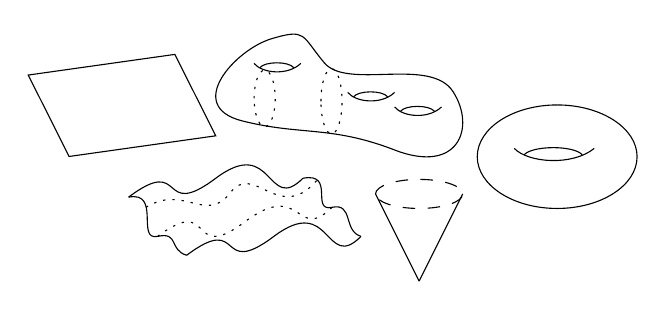
\begin{tikzpicture}[x=0.75pt,y=0.75pt,yscale=-0.7,xscale=0.7]
    %uncomment if require: \path (0,202); %set diagram left start at 0, and has height of 202
    
    %Curve Lines [id:da5236115066615021] 
    \draw    (375.49,78.68) .. controls (385.11,88.65) and (415.36,90.93) .. (430.49,78.68) ;
    %Curve Lines [id:da7101991261257758] 
    \draw    (422.24,82.95) .. controls (415.91,76.4) and (388.14,76.68) .. (382.36,82.95) ;
    %Shape: Ellipse [id:dp9157295048532674] 
    \draw   (350,84.38) .. controls (350,64.7) and (374.62,48.75) .. (405,48.75) .. controls (435.38,48.75) and (460,64.7) .. (460,84.38) .. controls (460,104.05) and (435.38,120) .. (405,120) .. controls (374.62,120) and (350,104.05) .. (350,84.38) -- cycle ;
    %Shape: Polygon Curved [id:ds6159505592009495] 
    \draw   (208.2,3.25) .. controls (232.62,-4.05) and (228.75,0.75) .. (244.72,19.75) .. controls (260.69,38.75) and (317.8,15.15) .. (333.44,39.75) .. controls (349.09,64.35) and (337.15,96.75) .. (293.11,79.75) .. controls (249.08,62.75) and (228.75,69.95) .. (188.26,59.75) .. controls (147.77,49.55) and (183.78,10.55) .. (208.2,3.25) -- cycle ;
    %Curve Lines [id:da5470586253636169] 
    \draw    (196.33,20.12) .. controls (201.97,27.12) and (219.72,28.72) .. (228.59,20.12) ;
    %Curve Lines [id:da010111340882360542] 
    \draw    (223.75,23.12) .. controls (220.04,18.52) and (203.75,18.72) .. (200.36,23.12) ;
    %Curve Lines [id:da5844912655809358] 
    \draw    (260.85,40.12) .. controls (266.5,47.12) and (284.24,48.72) .. (293.11,40.12) ;
    %Curve Lines [id:da11520475628245719] 
    \draw    (288.28,43.12) .. controls (284.57,38.52) and (268.27,38.72) .. (264.88,43.12) ;
    %Curve Lines [id:da20029327068385938] 
    \draw    (293.11,50.12) .. controls (298.76,57.12) and (316.5,58.72) .. (325.38,50.12) ;
    %Curve Lines [id:da040106671156743934] 
    \draw    (320.54,53.12) .. controls (316.83,48.52) and (300.53,48.72) .. (297.15,53.12) ;
    %Shape: Parallelogram [id:dp5212701228907126] 
    \draw   (40.94,28.18) -- (141.87,13.96) -- (170,70) -- (69.07,84.22) -- cycle ;
    %Curve Lines [id:da9139712577644594] 
    \draw    (110,112.22) .. controls (150,82.22) and (130,129.22) .. (170,99.22) .. controls (210,69.22) and (205,124.22) .. (230,99.22) ;
    %Curve Lines [id:da7132152828416398] 
    \draw    (150,152.22) .. controls (190,122.22) and (170,169.22) .. (210,139.22) .. controls (250,109.22) and (245,164.22) .. (270,139.22) ;
    %Curve Lines [id:da7754830305851486] 
    \draw    (110,112.22) .. controls (132.5,107.97) and (115,142.47) .. (130,139.22) .. controls (145,135.97) and (137.5,148.47) .. (150,152.22) ;
    %Curve Lines [id:da594486777960795] 
    \draw    (230,99.22) .. controls (252.5,94.97) and (235,122.47) .. (250,119.22) .. controls (265,115.97) and (257.5,135.47) .. (270,139.22) ;
    %Curve Lines [id:da5052126741414245] 
    \draw  [dash pattern={on 0.84pt off 2.51pt}]  (130,139.22) .. controls (170,109.22) and (150,159.22) .. (190,129.22) .. controls (230,99.22) and (225,144.22) .. (250,119.22) ;
    %Curve Lines [id:da3191700592357998] 
    \draw  [dash pattern={on 0.84pt off 2.51pt}]  (122,119.22) .. controls (148,102.97) and (163.5,130.97) .. (180,109.22) .. controls (196.5,87.47) and (213.5,131.47) .. (240,100.22) ;
    %Shape: Ellipse [id:dp5455375672721312] 
    \draw  [dash pattern={on 0.84pt off 2.51pt}] (242.41,46.25) .. controls (242.41,33.82) and (245.66,23.75) .. (249.67,23.75) .. controls (253.67,23.75) and (256.92,33.82) .. (256.92,46.25) .. controls (256.92,58.67) and (253.67,68.75) .. (249.67,68.75) .. controls (245.66,68.75) and (242.41,58.67) .. (242.41,46.25) -- cycle ;
    %Shape: Ellipse [id:dp7528987294411815] 
    \draw  [dash pattern={on 0.84pt off 2.51pt}] (196.43,44.25) .. controls (196.43,33.48) and (199.68,24.75) .. (203.69,24.75) .. controls (207.7,24.75) and (210.95,33.48) .. (210.95,44.25) .. controls (210.95,55.02) and (207.7,63.75) .. (203.69,63.75) .. controls (199.68,63.75) and (196.43,55.02) .. (196.43,44.25) -- cycle ;
    %Shape: Ellipse [id:dp915900620670441] 
    \draw  [dash pattern={on 4.5pt off 4.5pt}] (280,110) .. controls (280,104.48) and (293.43,100) .. (310,100) .. controls (326.57,100) and (340,104.48) .. (340,110) .. controls (340,115.52) and (326.57,120) .. (310,120) .. controls (293.43,120) and (280,115.52) .. (280,110) -- cycle ;
    %Straight Lines [id:da8069294757540748] 
    \draw    (280,110) -- (310,170) ;
    %Straight Lines [id:da5092407774777901] 
    \draw    (340,110) -- (310,170) ;
    
    
    
    
    \end{tikzpicture}
    
    \end{center}

We really care about surfaces where, in a sufficiently small region around each point, things look like we are in normal flat Euclidean space. This, along with a desire for things to be nice and smooth (as we shall define) will manifest into our basic notion of a \emph{manifold}.

\begin{definition}[Smooth]
    For an open subset $U \subseteq \R^n$, we say a function $f: U \rightarrow \R^m$ is \vocab{smooth}\footnote{For a function $f: X \rightarrow \R^m$ with $X$ not open, we say that $f$ is smooth if the above definition holds for some open neighborhood $V_x$ containing $x$ for each $x \in X$.} if it has continuous partial derivatives of all orders. 
\end{definition}

\begin{definition}[Diffeomorphism]
    A smooth function $f: X \rightarrow Y$ is a \vocab{diffeomorphism} if it's a bijection with smooth inverse. If a diffeomorphism between $X$ and $Y$ exists we say they are \vocab{diffeomorphic}.
\end{definition}

\begin{definition}[Manifold]
    We say that $X \subseteq \R^n$ is a \vocab{$k$-dimensional manifold} if each $x \in X$ has a neighborhood $V \subseteq X$ diffeomorphic to an open set of $\R^k$. 
\end{definition}

With neighborhoods around each point looking like $\R^k$, we can sensibly imagine that one could locally put a coordinate system on such neighborhoods, one coming from the diffeomorphism to $\R^k$. This motivates the definition of a \emph{chart} on a manifold.

\begin{center}
    

\tikzset{every picture/.style={line width=0.75pt}} %set default line width to 0.75pt        

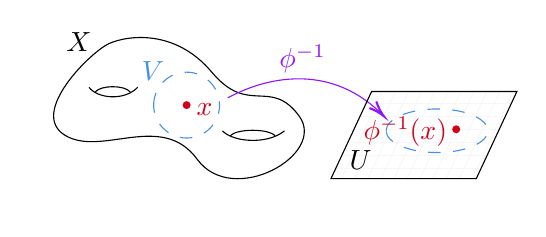
\begin{tikzpicture}[x=0.75pt,y=0.75pt,yscale=-0.7,xscale=0.7]
%uncomment if require: \path (0,315); %set diagram left start at 0, and has height of 315

%Shape: Grid [id:dp2824817026261346] 
\draw  [draw opacity=0] (409.35,113.32) -- (510,113.32) -- (482.02,173.32) -- (381.37,173.32) -- cycle ; \draw  [color={rgb, 255:red, 235; green, 235; blue, 235 }  ,draw opacity=0.39 ] (417.35,113.32) -- (389.37,173.32)(426.35,113.32) -- (398.37,173.32)(435.35,113.32) -- (407.37,173.32)(444.35,113.32) -- (416.37,173.32)(453.35,113.32) -- (425.37,173.32)(462.35,113.32) -- (434.37,173.32)(471.35,113.32) -- (443.37,173.32)(480.35,113.32) -- (452.37,173.32)(489.35,113.32) -- (461.37,173.32)(498.35,113.32) -- (470.37,173.32)(507.35,113.32) -- (479.37,173.32) ; \draw  [color={rgb, 255:red, 235; green, 235; blue, 235 }  ,draw opacity=0.39 ] (405.62,121.32) -- (506.27,121.32)(401.43,130.32) -- (502.07,130.32)(397.23,139.32) -- (497.88,139.32)(393.03,148.32) -- (493.68,148.32)(388.84,157.32) -- (489.48,157.32)(384.64,166.32) -- (485.29,166.32) ; \draw  [color={rgb, 255:red, 235; green, 235; blue, 235 }  ,draw opacity=0.39 ]  ;
%Shape: Polygon Curved [id:ds10590282788241523] 
\draw   (229.18,80.36) .. controls (241.44,74.78) and (274.67,69.76) .. (300,100) .. controls (325.33,130.24) and (340.15,103.45) .. (360,130) .. controls (379.85,156.55) and (314.5,193.47) .. (290,160) .. controls (265.5,126.53) and (224.14,158.79) .. (198.9,143.39) .. controls (173.66,128) and (216.93,85.94) .. (229.18,80.36) -- cycle ;
%Curve Lines [id:da5406567027069826] 
\draw    (215.5,110.42) .. controls (221.36,118.23) and (239.79,120.01) .. (249,110.42) ;
%Curve Lines [id:da11605042813104172] 
\draw    (243.97,113.77) .. controls (240.12,108.63) and (223.2,108.86) .. (219.69,113.77) ;
%Curve Lines [id:da8421916068847695] 
\draw    (307.33,140.42) .. controls (314.8,148.23) and (338.27,150.01) .. (350,140.42) ;
%Curve Lines [id:da5979992538827481] 
\draw    (343.6,143.77) .. controls (338.69,138.63) and (317.14,138.86) .. (312.66,143.77) ;
%Shape: Circle [id:dp7284538694447111] 
\draw  [draw opacity=0][fill={rgb, 255:red, 208; green, 2; blue, 27 }  ,fill opacity=1 ] (279.92,122.67) .. controls (279.92,121.15) and (281.15,119.92) .. (282.67,119.92) .. controls (284.19,119.92) and (285.42,121.15) .. (285.42,122.67) .. controls (285.42,124.19) and (284.19,125.42) .. (282.67,125.42) .. controls (281.15,125.42) and (279.92,124.19) .. (279.92,122.67) -- cycle ;
%Shape: Circle [id:dp8388763618077151] 
\draw  [color={rgb, 255:red, 74; green, 144; blue, 226 }  ,draw opacity=1 ][dash pattern={on 4.5pt off 4.5pt}] (260,122.67) .. controls (260,110.15) and (270.15,100) .. (282.67,100) .. controls (295.19,100) and (305.33,110.15) .. (305.33,122.67) .. controls (305.33,135.19) and (295.19,145.33) .. (282.67,145.33) .. controls (270.15,145.33) and (260,135.19) .. (260,122.67) -- cycle ;
%Curve Lines [id:da4312845382129431] 
\draw [color={rgb, 255:red, 144; green, 19; blue, 254 }  ,draw opacity=1 ]   (311,117.68) .. controls (341.69,101.07) and (384.23,95.68) .. (417.42,129.29) ;
\draw [shift={(418.43,130.32)}, rotate = 226.19] [color={rgb, 255:red, 144; green, 19; blue, 254 }  ,draw opacity=1 ][line width=0.75]    (10.93,-3.29) .. controls (6.95,-1.4) and (3.31,-0.3) .. (0,0) .. controls (3.31,0.3) and (6.95,1.4) .. (10.93,3.29)   ;
%Shape: Ellipse [id:dp020561129589376614] 
\draw  [color={rgb, 255:red, 74; green, 144; blue, 226 }  ,draw opacity=1 ][dash pattern={on 4.5pt off 4.5pt}] (420,140.32) .. controls (420,132.04) and (435.67,125.32) .. (455,125.32) .. controls (474.33,125.32) and (490,132.04) .. (490,140.32) .. controls (490,148.61) and (474.33,155.32) .. (455,155.32) .. controls (435.67,155.32) and (420,148.61) .. (420,140.32) -- cycle ;
%Shape: Rectangle [id:dp6823458888863583] 
\draw   (410,113.32) -- (510,113.32) -- (482.02,173.32) -- (382.02,173.32) -- cycle ;
%Shape: Circle [id:dp01371884157878056] 
\draw  [draw opacity=0][fill={rgb, 255:red, 208; green, 2; blue, 27 }  ,fill opacity=1 ] (465.48,139.32) .. controls (465.48,137.8) and (466.71,136.57) .. (468.23,136.57) .. controls (469.75,136.57) and (470.98,137.8) .. (470.98,139.32) .. controls (470.98,140.84) and (469.75,142.07) .. (468.23,142.07) .. controls (466.71,142.07) and (465.48,140.84) .. (465.48,139.32) -- cycle ;

% Text Node
\draw (287.75,125.75) node [anchor=west] [inner sep=0.75pt]  [color={rgb, 255:red, 208; green, 2; blue, 27 }  ,opacity=1 ]  {$x$};
% Text Node
\draw (269,107.6) node [anchor=south east] [inner sep=0.75pt]  [color={rgb, 255:red, 74; green, 144; blue, 226 }  ,opacity=1 ]  {$V$};
% Text Node
\draw (219,87.6) node [anchor=south east] [inner sep=0.75pt]    {$X$};
% Text Node
\draw (362.5,102.6) node [anchor=south] [inner sep=0.75pt]  [color={rgb, 255:red, 144; green, 19; blue, 254 }  ,opacity=1 ]  {$\phi^{-1} $};
% Text Node
\draw (393,152.4) node [anchor=north west][inner sep=0.75pt]    {$U$};
% Text Node
\draw (463.75,141.07) node [anchor=east] [inner sep=0.75pt]  [color={rgb, 255:red, 208; green, 2; blue, 27 }  ,opacity=1 ]  {$\phi^{-1} (x)$};


\end{tikzpicture}

\end{center}

\begin{definition}[Chart]
    A diffeomorphism $\phi: U \rightarrow V$, where $U$ is an open set of $\R^k$ is a \vocab{parameterisation} of the neighborhood $V$. The inverse diffeomorphism $\phi^{-1}: V \rightarrow U$ is called a \vocab{chart} on $V$.
\end{definition}

Of course, if we have manifolds $X$ and $Z$ with $Z \subseteq X$ we say that $Z$ is a \vocab{submanifold} of $X$. In this case, the \vocab{codimension} of $Z$ in $X$ is $\dim X - \dim Z$.

\subsection{Tangent Spaces and Derivatives}

This is a course in differential geometry, and we've pinned down the `geometry' part, now it's time to pin down the `differential part'. We want to generalise the notion of a derivative for smooth functions on manifolds. 

The idea you should have in your head of derivatives are that they are the best linear approximation to a given function. From this perspective, defining the derivative on manifolds requires us to answer two questions: 
what space should be our `linear approximation' to a manifold that our derivative should act on, and then what is our linear approximation? Answering the first of these questions will lead us to the notion of \vocab{tangent spaces}.

\begin{center}


% Gradient Info
  
\tikzset {_a105vjgip/.code = {\pgfsetadditionalshadetransform{ \pgftransformshift{\pgfpoint{89.1 bp } { -128.7 bp }  }  \pgftransformscale{1.32 }  }}}
\pgfdeclareradialshading{_rvjpvtrtp}{\pgfpoint{-72bp}{104bp}}{rgb(0bp)=(1,1,1);
rgb(0bp)=(1,1,1);
rgb(25bp)=(0.78,0.88,1);
rgb(400bp)=(0.78,0.88,1)}
\tikzset{every picture/.style={line width=0.75pt}} %set default line width to 0.75pt        
\Small
\begin{tikzpicture}[x=0.75pt,y=0.75pt,yscale=-0.5,xscale=0.5]
%uncomment if require: \path (0,459); %set diagram left start at 0, and has height of 459

%Shape: Ellipse [id:dp9362732221206294] 
\path  [shading=_rvjpvtrtp,_a105vjgip] (286.32,142.35) .. controls (286.32,106.85) and (315.03,78.07) .. (350.45,78.07) .. controls (385.87,78.07) and (414.59,106.85) .. (414.59,142.35) .. controls (414.59,177.85) and (385.87,206.63) .. (350.45,206.63) .. controls (315.03,206.63) and (286.32,177.85) .. (286.32,142.35) -- cycle ; % for fading 
 \draw   (286.32,142.35) .. controls (286.32,106.85) and (315.03,78.07) .. (350.45,78.07) .. controls (385.87,78.07) and (414.59,106.85) .. (414.59,142.35) .. controls (414.59,177.85) and (385.87,206.63) .. (350.45,206.63) .. controls (315.03,206.63) and (286.32,177.85) .. (286.32,142.35) -- cycle ; % for border 

%Shape: Ellipse [id:dp05909251883009348] 
\draw  [dash pattern={on 0.84pt off 2.51pt}] (286.61,142.9) .. controls (286.61,132.73) and (315.33,124.49) .. (350.75,124.49) .. controls (386.17,124.49) and (414.88,132.73) .. (414.88,142.9) .. controls (414.88,153.06) and (386.17,161.3) .. (350.75,161.3) .. controls (315.33,161.3) and (286.61,153.06) .. (286.61,142.9) -- cycle ;
%Straight Lines [id:da9841679462645883] 
\draw    (271.39,41.76) -- (271.39,257.32) ;
\draw [shift={(271.39,259.32)}, rotate = 270] [color={rgb, 255:red, 0; green, 0; blue, 0 }  ][line width=0.75]    (10.93,-3.29) .. controls (6.95,-1.4) and (3.31,-0.3) .. (0,0) .. controls (3.31,0.3) and (6.95,1.4) .. (10.93,3.29)   ;
\draw [shift={(271.39,39.76)}, rotate = 90] [color={rgb, 255:red, 0; green, 0; blue, 0 }  ][line width=0.75]    (10.93,-3.29) .. controls (6.95,-1.4) and (3.31,-0.3) .. (0,0) .. controls (3.31,0.3) and (6.95,1.4) .. (10.93,3.29)   ;
%Straight Lines [id:da8789267641621146] 
\draw    (381.94,258.6) -- (205.63,189.79) ;
\draw [shift={(203.76,189.06)}, rotate = 21.32] [color={rgb, 255:red, 0; green, 0; blue, 0 }  ][line width=0.75]    (10.93,-3.29) .. controls (6.95,-1.4) and (3.31,-0.3) .. (0,0) .. controls (3.31,0.3) and (6.95,1.4) .. (10.93,3.29)   ;
\draw [shift={(383.81,259.32)}, rotate = 201.32] [color={rgb, 255:red, 0; green, 0; blue, 0 }  ][line width=0.75]    (10.93,-3.29) .. controls (6.95,-1.4) and (3.31,-0.3) .. (0,0) .. controls (3.31,0.3) and (6.95,1.4) .. (10.93,3.29)   ;
%Straight Lines [id:da6899728376032785] 
\draw    (438.96,172) -- (205.7,232.47) ;
\draw [shift={(203.76,232.98)}, rotate = 345.47] [color={rgb, 255:red, 0; green, 0; blue, 0 }  ][line width=0.75]    (10.93,-3.29) .. controls (6.95,-1.4) and (3.31,-0.3) .. (0,0) .. controls (3.31,0.3) and (6.95,1.4) .. (10.93,3.29)   ;
\draw [shift={(440.89,171.5)}, rotate = 165.47] [color={rgb, 255:red, 0; green, 0; blue, 0 }  ][line width=0.75]    (10.93,-3.29) .. controls (6.95,-1.4) and (3.31,-0.3) .. (0,0) .. controls (3.31,0.3) and (6.95,1.4) .. (10.93,3.29)   ;
%Shape: Parallelogram [id:dp9354673320662454] 
\draw  [fill={rgb, 255:red, 255; green, 179; blue, 179 }  ,fill opacity=0.55 ] (320.97,76.05) -- (395.78,65.51) -- (434.75,115.84) -- (359.94,126.38) -- cycle ;
%Shape: Ellipse [id:dp6082542857300584] 
\draw  [draw opacity=0][fill={rgb, 255:red, 208; green, 2; blue, 27 }  ,fill opacity=1 ] (373.27,93.97) .. controls (373.27,91.49) and (375.27,89.49) .. (377.74,89.49) .. controls (380.2,89.49) and (382.2,91.49) .. (382.2,93.97) .. controls (382.2,96.44) and (380.2,98.44) .. (377.74,98.44) .. controls (375.27,98.44) and (373.27,96.44) .. (373.27,93.97) -- cycle ;
%Shape: Parallelogram [id:dp02184396300423197] 
\draw  [fill={rgb, 255:red, 255; green, 179; blue, 179 }  ,fill opacity=0.55 ][dash pattern={on 0.84pt off 2.51pt}] (217.82,197.84) -- (292.62,187.3) -- (331.59,237.63) -- (256.79,248.17) -- cycle ;
%Curve Lines [id:da7874596527392925] 
\draw [color={rgb, 255:red, 74; green, 144; blue, 226 }  ,draw opacity=1 ]   (484.81,153.93) .. controls (455.54,171.41) and (432.18,158.27) .. (432.09,129.37) ;
\draw [shift={(432.11,127.58)}, rotate = 91.67] [color={rgb, 255:red, 74; green, 144; blue, 226 }  ,draw opacity=1 ][line width=0.75]    (10.93,-3.29) .. controls (6.95,-1.4) and (3.31,-0.3) .. (0,0) .. controls (3.31,0.3) and (6.95,1.4) .. (10.93,3.29)   ;
%Curve Lines [id:da12125466160712395] 
\draw [color={rgb, 255:red, 74; green, 144; blue, 226 }  ,draw opacity=1 ]   (405.76,224.19) .. controls (379.22,211.18) and (351,214.19) .. (328.44,223.47) ;
\draw [shift={(326.72,224.19)}, rotate = 336.7] [color={rgb, 255:red, 74; green, 144; blue, 226 }  ,draw opacity=1 ][line width=0.75]    (10.93,-3.29) .. controls (6.95,-1.4) and (3.31,-0.3) .. (0,0) .. controls (3.31,0.3) and (6.95,1.4) .. (10.93,3.29)   ;
%Shape: Parallelogram [id:dp6323732088439955] 
\draw   (14.47,104.75) -- (133.5,104.75) -- (202.35,153.93) -- (83.32,153.93) -- cycle ;
%Shape: Ellipse [id:dp013750574349542521] 
\draw  [draw opacity=0][fill={rgb, 255:red, 208; green, 2; blue, 27 }  ,fill opacity=1 ] (118.57,131.01) .. controls (118.57,128.54) and (120.57,126.53) .. (123.04,126.53) .. controls (125.51,126.53) and (127.51,128.54) .. (127.51,131.01) .. controls (127.51,133.48) and (125.51,135.49) .. (123.04,135.49) .. controls (120.57,135.49) and (118.57,133.48) .. (118.57,131.01) -- cycle ;
%Shape: Ellipse [id:dp307221795102091] 
\draw  [dash pattern={on 0.84pt off 2.51pt}] (89.59,131.54) .. controls (89.59,124.02) and (103.35,117.92) .. (120.33,117.92) .. controls (137.3,117.92) and (151.07,124.02) .. (151.07,131.54) .. controls (151.07,139.05) and (137.3,145.15) .. (120.33,145.15) .. controls (103.35,145.15) and (89.59,139.05) .. (89.59,131.54) -- cycle ;
%Curve Lines [id:da45072719289244145] 
\draw [color={rgb, 255:red, 144; green, 19; blue, 254 }  ,draw opacity=1 ]   (108.93,148.66) .. controls (99.46,180.78) and (167.59,234.3) .. (203.38,211.62) ;
\draw [shift={(205.53,210.14)}, rotate = 143.13] [fill={rgb, 255:red, 144; green, 19; blue, 254 }  ,fill opacity=1 ][line width=0.08]  [draw opacity=0] (8.93,-4.29) -- (0,0) -- (8.93,4.29) -- cycle    ;
%Curve Lines [id:da5468420319874947] 
\draw [color={rgb, 255:red, 144; green, 19; blue, 254 }  ,draw opacity=1 ]   (124.72,110.02) .. controls (175.15,59.87) and (245.38,40.43) .. (307.28,73.86) ;
\draw [shift={(309.16,74.89)}, rotate = 209.2] [fill={rgb, 255:red, 144; green, 19; blue, 254 }  ,fill opacity=1 ][line width=0.08]  [draw opacity=0] (8.93,-4.29) -- (0,0) -- (8.93,4.29) -- cycle    ;

% Text Node
\draw (362,81.01) node [anchor=north west] [color={rgb, 255:red, 0; green, 0; blue, 0 }  ,opacity=1 ]  {$x$};
% Text Node
\draw (381.09,46.64) node [anchor=north west]  [color={rgb, 255:red, 0; green, 0; blue, 0 }  ,opacity=1 ]  {$x+T_{x} X$};
% Text Node
\draw (282.83,91.55) node [anchor=north west]  [color={rgb, 255:red, 0; green, 0; blue, 0 }  ,opacity=1 ]  {$X$};
% Text Node
\draw (229.04,171.68) node [anchor=north west]  [color={rgb, 255:red, 0; green, 0; blue, 0 }  ,opacity=1 ]  {$T_{x} X$};
% Text Node
\draw (111.25,202.42) node [anchor=north west]  [color={rgb, 255:red, 144; green, 19; blue, 254 }  ,opacity=1 ]  {$D_{0} \phi $};
% Text Node
\draw (442.34,136.21) node [anchor=north west]  [color={rgb, 255:red, 74; green, 144; blue, 226 }  ,opacity=1 ] [align=left] {Affine tangent plane};
% Text Node
\draw (391.77,233.7) node [anchor=north west]  [color={rgb, 255:red, 74; green, 144; blue, 226 }  ,opacity=1 ] [align=left] {Tangent space};
% Text Node
\draw (71.99,119.98) node [anchor=north west]    {$U$};
% Text Node
\draw (186.88,39.06) node [anchor=north west]  [color={rgb, 255:red, 144; green, 19; blue, 254 }  ,opacity=1 ]  {$x+D_{0} \phi $};


\end{tikzpicture}
    
\end{center}

% For any open set $U \subseteq \R^n$ and $x \in U$, the \vocab{tangent space} to $U$ at $x$ is defined to be $\R^n$. We generalise this to manifolds with the following.

\begin{definition}[Tangent Space of a Manifold]
    Let $X \subseteq \R^n$ be an arbitrary smooth manifold, and let $x \in X$. Choose a parameterisation $\phi: U \rightarrow X$ with $\phi(0) = x$ where $U$ is an open set of $\R^k$. Then thinking of $\phi$ as a map from $U$ to $\R^N$, we define the \vocab{tangent space} $T_x X$ to be the image of the derivative of $\phi$ at $0$, $D_{0} \phi(\R^k)$. 
\end{definition}

In this definition we had to pick some parameterisation $\phi$, but one would hope that our resulting space is independent of this choice. Indeed, this is the case.

\begin{lemma}[Tangent Spaces are Paramaterisation Independent]
    $T_x X$ does not depend on the parameterisation $\phi$ chosen.
\end{lemma}
\begin{proof}
    Suppose $\psi: V \rightarrow X$ is another choice of parameteristaion, and suppose without loss of generality that $\phi(0) = \psi(0) = x$.
    By shrinking both $U$ and $V$, we may assume that $\phi(U)=\psi(V)$. Then the map $h=\psi^{-1} \circ \phi$ : $U \rightarrow V$ is a diffeomorphism. Now we write $\phi=\psi \circ h$ and we differentiate. Using the chain rule we have: $D_0 \phi =D_0 \psi \circ D_0 h$. Since $D_0 h$ is an invertible linear map, it follows at once that $D_0 \phi$ and $D_0 \psi$ have the same image.
\end{proof}

We are now ready to define the derivative of a smooth map $f: X \rightarrow Y$ between arbitrary manifolds, and we will see that it comes rather naturally. We would hope that for $X$ and $Y$ open subsets of euclidean space, our new definition should coincide with our previous definition of the derivative. Also, we would expect that the chain rule should still hold. This is going to force our definition.

Let $\phi: U \rightarrow X$ and $\psi: V \rightarrow Y$ be parameterisations, with $\phi(0) = x$, $\psi(0) = y$ and $U, V$ being open subsets of $\R^k$ and $\R^l$ respectively. Then for small enough $U$, the following diagram commutes:

% https://q.uiver.app/?q=WzAsNCxbMCwwLCJYIl0sWzIsMCwiWSJdLFswLDEsIlUiXSxbMiwxLCJWIl0sWzAsMSwiZiJdLFsyLDAsIlxccGhpIl0sWzMsMSwiXFxwc2kiLDJdLFsyLDMsImg9XFxwc2leey0xfSBcXGNpcmMgZiBcXGNpcmMgXFxwaGkiXV0=
\[\begin{tikzcd}
	X && Y \\
	U && V
	\arrow["f", from=1-1, to=1-3]
	\arrow["\phi", from=2-1, to=1-1]
	\arrow["\psi"', from=2-3, to=1-3]
	\arrow["{h=\psi^{-1} \circ f \circ \phi}", from=2-1, to=2-3]
\end{tikzcd}\]

Then $D_0 \psi$, $D_0 \phi$, $D_0 h$ are all well defined, and as we said previously we would hope the chain rule still holds, which implies that the following square of linear maps commutes:

% https://q.uiver.app/?q=WzAsNCxbMCwwLCJUX3hYIl0sWzIsMCwiVF95WSJdLFswLDEsIlxcUl5rIl0sWzIsMSwiXFxSXmwiXSxbMCwxLCJkZl94Il0sWzIsMCwiZFxccGhpXzAiXSxbMywxLCJkXFxwc2lfMCIsMl0sWzIsMywiZGhfMCJdXQ==
\[\begin{tikzcd}
	{T_xX} && {T_yY} \\
	{\R^k} && {\R^l}
	\arrow["{df_x}", from=1-1, to=1-3]
	\arrow["{d\phi_0}", from=2-1, to=1-1]
	\arrow["{d\psi_0}"', from=2-3, to=1-3]
	\arrow["{dh_0}", from=2-1, to=2-3]
\end{tikzcd}\]

Then since $D_0 \phi$ is an isomorphism, only one definition of $D_x f$ will meet our requirements, namely
$$
D_x f = D_0 \psi \circ D_0 h \circ D_0 \phi^{-1}.
$$

Again, one would hope that this definition of $D_x f$ is independent of $\phi$ and $\psi$, and this is the case (and the same proof as before works). Also, we have forced the chain rule still to hold.

\begin{theorem}[Chain Rule]
    If $f: X \rightarrow Y$ and $g: Y \rightarrow Z$ are smooth maps between manifolds, then
    $$
    D_x(g \circ f) = D_{f(x)} g \circ D_x f.
    $$
\end{theorem}
\begin{proof}
    Omitted.
\end{proof}


\subsubsection{The Inverse Function Theorem}

Let $f: X \rightarrow Y$ be a smooth map between manifolds. We say that $f$ is a \vocab{local diffeomorphism} at $x$ if $f$ maps a neighbourhood of $x$ diffeomorphically onto a neighbourhood of $f(x)$.

\begin{theorem}[Inverse Function Theorem]
    Suppose that $f: X \rightarrow Y$ is a smooth map whose derivative $d f_{x}$ at the point $x$ is an isomorphism. Then $f$ is a local diffeomorphism at $x$.
\end{theorem}
\begin{proof}[Proof Sketch]
    This can be proven using the inverse function theorem for smooth functions between open sets of Euclidean space, as was shown in Analysis II.
\end{proof}


\subsection{Regular values and Sard's theorem}
Let $f: X \rightarrow Y$ be a smooth map between manifolds. Let $C$ be the set of all points $x \in X$ such that $d f_{x}: T_{x} X \rightarrow T_{f(x)} Y$ is not surjective.

\begin{definition}
    A point in $C$ will be called a \vocab{critical point}. A point in $f(C)$ will be called a \vocab{critical value}. A point in the complement of $f(C)$ will be called a \vocab{regular value}.
\end{definition}

\begin{remark}
    Note that if $\operatorname{dim} X<\operatorname{dim} Y$, then $C=X$ and the preimage of a regular value is the empty set.
\end{remark}

\begin{theorem}[Preimage Theorem]
    Let y be a regular value of $f: X \rightarrow Y$ with $\operatorname{dim} X \geq \operatorname{dim} Y$. Then the set $f^{-1}(y)$ is a submanifold of $X$ with $\operatorname{dim} f^{-1}(y)=$ $\operatorname{dim} X-\operatorname{dim} Y$.
\end{theorem}
\begin{proof}
    Let $x \in f^{-1}(y)$. Since $y$ is a regular value, the derivative $d f_{x}$ maps $T_{x} X$ onto $T_{y} Y$. The kernel of $d f_{x}$ is a subspace $K$ of $T_{x} X$ of dimension $p:=$ $\operatorname{dim} X-\operatorname{dim} Y$. Suppose $X \subset \mathbb{R}^{N}$ and let $T: \mathbb{R}^{N} \rightarrow \mathbb{R}^{p}$ be any linear map such that $\operatorname{Ker}(T) \cap K=\{0\}$. Consider the map $F: X \rightarrow Y \times \mathbb{R}^{p}$ given by
$$
F(z)=(f(z), T(z)).
$$
The derivative of $F$ is given by
$$
d F_{x}(v)=\left(d f_{x}(v), T(v)\right)
$$
which is clearly nonsingular by our choice of $T$. By the inverse function theorem, $F$ is a local diffeomorphism at $x$, i.e. $F$ maps some neighbourhood $U$ of $x$ diffeomorphically onto a neighbourhood $V$ of $(y, T(x))$. Hence $F$ maps $f^{-1}(y) \cap U$ diffeomorphically onto $\left(\{y\} \times \mathbb{R}^{p}\right) \cap V$ which proves that $f^{-1}(y)$ is a manifold with $\operatorname{dim} f^{-1}(y)=p$.
\end{proof}

The case $\operatorname{dim} X=\operatorname{dim} Y$ is particularly important. The theorem says that if $y$ is a regular value of $f$, then $f^{-1}(y)$ is a 0 -dimensional manifold, i.e. collection of points. If $X$ is compact, this collection must be finite (why?) so we obtain:

\begin{corollary}
    Let $f: X \rightarrow Y$ be a smooth map between manifolds of the same dimension. If $X$ is compact and $y$ is a regular value, $f^{-1}(y)$ consists of a finite set of points.
\end{corollary}

We can actually say a bit more:

\begin{theorem}[Stack of Records Theorem]
    Let $f: X \rightarrow Y$ be a smooth map between manifolds of the same dimension with $X$ compact. Let y be a regular value of $f$ and write $f^{-1}(y)=\left\{x_{1}, \ldots, x_{k}\right\}$. Then there exists a neighbourhood $U$ of $y$ in $Y$ such that $f^{-1}(U)$ is a disjoint union $V_{1} \cup \cdots \cup V_{k}$, where $V_{i}$ is an open neighbourhood of $x_{i}$ and $f$ maps each $V_{i}$ diffeomorphically onto $U$.
\end{theorem}
\begin{proof}
    By the inverse function theorem we can pick disjoint neighbourhoods $W_{i}$ of $x_{i}$ such that $f$ maps $W_{i}$ diffeomorphically onto a neighbourhood of $y$. Observe that $f\left(X-\cup_{i} W_{i}\right)$ is a compact set which does not contain $y$. Now take
$$
U:=\cap_{i} f\left(W_{i}\right)-f\left(X-\cup_{i} W_{i}\right).
$$
\end{proof}


If we let $\# f^{-1}(y)$ be the cardinality of $f^{-1}(y)$, the theorem implies that the function $y \mapsto \# f^{-1}(y)$ is locally constant as $y$ ranges over regular values of $f$.

The Preimage theorem gives a particularly nice way of producing manifolds. For example, if we consider the map $f: \mathbb{R}^{n+1} \rightarrow \mathbb{R}$ given by $f(x)=|x|^{2}$ we can check easily that 1 is a regular value of $f$ (do it!). Hence $S^{n}=f^{-1}(1)$ is a smooth manifold of dimension $n$. By switching our mental wavelength a little we can produce quite interesting examples as follows:

\begin{example}[Orthogonal Group]
    Let $O(n)$ be the group of orthogonal matrices of size $n \times n$, i.e., a matrix $A \in O(n)$ if and only if $A A^{t}=I$, where $I$ is the identity matrix. The space of all $n \times n$
matrices $M(n)$ is just $\mathbb{R}^{n^{2}}$, so we can think of $O(n)$ as living inside $\mathbb{R}^{n^{2}}$. We will show that $O(n)$ is a manifold of dimension $\frac{n(n-1)}{2}$.

Let $S(n) \subset M(n)$ be the space of all symmetric matrices. Since it is a vector space, is clearly a submanifold of $M(n)$ and it has dimension $\frac{n(n+1)}{2}$.

Let $f: M(n) \rightarrow S(n)$ be the smooth map $f(A)=A A^{t}$. Since $O(n)=f^{-1}(I)$ it suffices to show that $I$ is a regular value of $f$. We compute:
$$
\begin{aligned}
d f_{A}(H) & =\lim _{s \rightarrow 0} \frac{f(A+s H)-f(A)}{s} \\
& =\lim _{s \rightarrow 0} \frac{(A+s H)(A+s H)^{t}-A A^{t}}{s} \\
& =H A^{t}+A H^{t}.
\end{aligned}
$$
Fix $A$ with $A A^{t}=I$. We must prove that given any $C \in S(n)=T_{I} S(n)$ there is $H \in M(n)=T_{A} M(n)$ such that
$$
d f_{A}(H)=H A^{t}+A H^{t}=C.
$$
Since $C$ is symmetric, we can write $C=\frac{1}{2} C+\frac{1}{2} C^{t}$ so if we can solve $H A^{t}=\frac{1}{2} C$ we are done. Multiplying by $A$ on the right and using $A A^{t}=I$ we obtain $H=\frac{1}{2} C A$ which solves $d f_{A}(H)=C$. Thus $I$ is a regular value of $f$.

Note that $O(n)$ is both a group and a manifold. In fact, the group operations are smooth, that is, the maps $(A, B) \mapsto A B$ and $A \mapsto A^{-1}=A^{t}$ are smooth. (Why?) A group that is manifold, and whose group operations are smooth, is called a Lie group.
\end{example}

\subsubsection{Sard's Theorem}

The Preimage theorem raises the question: is it easy to find regular values? How are abundant are they?

Recall that an arbitrary set $A$ in $\mathbb{R}^{n}$ has measure zero if it can be covered by a countable number of rectangular solids with arbitrary small total volume. In other words given $\varepsilon>0$, there exists a countable collection $\left\{R_{1}, R_{2}, \ldots\right\}$ of rectangular solids in $\mathbb{R}^{n}$, such that $A$ is contained in $\cup_{i} R_{i}$ and
$$
\sum_{i} \operatorname{Vol}\left(R_{i}\right)<\varepsilon \text {. }
$$
Let $X$ be manifold. An arbitrary subset $A \subset X$ has \vocab{measure zero} if, for every local parametrization $\phi$ of $X, \phi^{-1}(A)$ has measure zero in Euclidean space.

The following deep theorem, tells us that there are plenty of regular values.

\begin{theorem}[Sard's Theorem, 1942]
    The set of critical values of a smooth map $f: X \rightarrow Y$ has measure zero.
\end{theorem}

Since a set of measure zero cannot contain a non-empty open set we obtain:

\begin{corollary}
    The regular values of any smooth map $f: X \rightarrow Y$ are dense in $Y$.
\end{corollary}

\subsubsection{Morse Functions}

See the first example sheet.


\subsection{Transversality}

We know that the solutions of the equation $f(x)=y$ form a smooth manifold, provided that $y$ is a regular value of $f: X \rightarrow Y$. Suppose now that we replace $y$ by a submanifold $Z \subset Y$ and we ask, when is $f^{-1}(Z)$ a submanifold of $X$ ?

\begin{definition}[Transversal]
    A smooth map $f: X \rightarrow Y$ is said to be \vocab{transversal} to a submanifold $Z \subset Y$ if for every $x \in f^{-1}(Z)$ we have
$$
\operatorname{Image}\left(d f_{x}\right)+T_{f(x)} Z=T_{f(x)} Y.
$$
We write $f \pitchfork Z$.
\end{definition}

Note that if $Z=\{y\}$, the notion of transversality reduces to the notion of regular value.

With this definition, we can now state a more general version of the Preimage theorem.

\begin{theorem}
    If the smooth map $f: X \rightarrow Y$ is transversal to a submanifold $Z \subset Y$, then $f^{-1}(Z)$ is submanifold of $X$. Moreover, $f^{-1}(Z)$ and $Z$ have the same codimension.
\end{theorem}
\begin{proof}[Proof (Non-examinable, sketch only)]
    It is not hard to see that $Z$ can be written in a neighbourhood of a point $y=f(x)$ as the zero set of a collection of functions $h_{1}, \ldots, h_{r}$, where $r$ is the codimension of $Z$ in $Y$. Let $H:=\left(h_{1}, \ldots, h_{r}\right)$. Then near $x, f^{-1}(Z)$ is the zero set of the function $H \circ f$. Thus if $0 \in \mathbb{R}^{r}$ is a regular value of $H \circ f$ we are done. But $d H_{y} \circ d f_{x}$ is surjective if and only if
    $$
    \operatorname{Image}\left(d f_{x}\right)+T_{f(x)} Z=T_{f(x)} Y
    $$
    since $d H_{y}: T_{y} Y \rightarrow \mathbb{R}^{r}$ is onto with kernel $T_{y} Z$.
\end{proof}

\begin{example}
    Consider $f: \mathbb{R} \rightarrow \mathbb{R}^{2}$ given by $f(t)=(0, t)$ and let $Z$ be the $x$ axis in $\mathbb{R}^{2}$. Then $f$ is transversal to $Z$, but for example the map $h(t)=\left(t, t^{2}\right)$ is not.
\end{example}

An important special case occurs when $f$ is the inclusion of a submanifold $X$ of $Y$ and $Z$ is another submanifold of $Y$. In this case the condition of transversality reduces to
$$
T_{x} X+T_{x} Z=T_{x} Y
$$
for every $x \in X \cap Z$. This condition is quite easy to visualize and when it holds we say that $X$ and $Z$ are transversal (we write $X \pitchfork Z$). We now have:

\begin{theorem}
    The intersection of two transversal submanifolds of $Y$ is a submanifold of codimension given by
$$
\operatorname{codim}(X \cap Z)=\operatorname{codim} X+\operatorname{codim} Z.
$$
\end{theorem}

One of the main virtues of the notion of transversality is its stability i.e. it survives after small perturbations of the map $f$. You can convince yourself of this property by looking at pictures of transversal submanifolds of Euclidean space. Another very important virtue is genericity: smooth maps may be deformed by arbitrary small amounts into a map that is transversal to $Z$. (This is non-obvious and we refer to Chapter 2 in the book by Guillemin and Pollack for details.)

\subsection{Manifolds with Boundary}

Consider the closed half-space
$$
\mathbb{H}^{k}:=\left\{\left(x_{1}, \ldots, x_{k}\right) \in \mathbb{R}^{k}: x_{k} \geq 0\right\}.
$$
The boundary $\partial \mathbb{H}^{n}$ is defined to be the hyperplane $x_{k}=0$ in $\mathbb{R}^{k}$.

\begin{definition}
    A subset $X \subset \mathbb{R}^{N}$ is called a smooth $k$-manifold with boundary if each $x \in X$ has a neighbourhood diffeomorphic to an open set in $\mathbb{H}^{k}$. As before, such a diffeomorphism is called a chart on $X$. The boundary of $X$, denoted $\partial X$, is given by the set of points that belong to the image of $\partial \mathbb{H}^{k}$ under some local parametrization. Its complement is called the interior of $X$, $\operatorname{Int}(X)=X-\partial X$.
\end{definition}

\begin{remark}[Warning]
    Do not confuse the boundary or interior of $X$ as defined above with the topological notions of interior and boundary as a subset of $\mathbb{R}^{N}$.
\end{remark}


The tangent space is defined as before, so that $T_{x} X$ is a $k$-dimensional vector space even for points $x \in \partial X$. The interior of $X$ is a $k$-manifold without boundary and $\partial X$ is a manifold without boundary of dimension $k-1$ (this requires a proof!).

Here is an easy way of generating examples.

\begin{lemma}
    Let $X$ be a manifold without boundary and let $f: X \rightarrow \mathbb{R}$ be $a$ smooth function with 0 as a regular value. Then the subset $\{x \in X: f(x) \geq 0\}$ is a smooth manifold with boundary equal to $f^{-1}(0)$.
\end{lemma}
\begin{proof}
    The set where $f>0$ is open in $X$ and is therefore a submanifold of the same dimension as $X$. For a point $x \in X$ with $f(x)=0$, the same proof of the Preimage Theorem $1.13$ shows that $x$ has a neighbourhood diffeomorphic to a neighbourhood of a point in $\mathbb{H}^{k}$.
\end{proof}

As an easy application of the lemma, consider the unit ball $B^{k}$ given by all $x \in \mathbb{R}^{k}$ such that $|x| \leq 1$. By considering the function $f(x)=1-|x|^{2}$ it follows that $B^{k}$ is a smooth manifold with boundary $S^{k-1}$.

\begin{theorem}
    Let $f: X \rightarrow Y$ be a smooth map from an m-manifold with boundary to an $n$-manifold, where $m>n$. If $y$ is a regular value, both for $f$ and for the restriction of $f$ to $\partial X$, then $f^{-1}(y)$ is a smooth $(m-n)$-manifold with boundary equal to $f^{-1}(y) \cap \partial X$
\end{theorem}
\begin{proof}
    Recall that being a submanifold is a local property so without loss of generality we can suppose that $f: \mathbb{H}^{m} \rightarrow \mathbb{R}^{n}$ with $y \in \mathbb{R}^{n}$ a regular value. Consider $z \in f^{-1}(y)$. If $z$ belongs to the interior of $\mathbb{H}^{m}$, then as in the Preimage theorem $1.13 f^{-1}(y)$ is a smooth manifold near $z$.

Let $z$ be now in $\partial \mathbb{H}^{m}$. Since $f$ is smooth, there is a neighbourhood $U$ of $z$ in $\mathbb{R}^{m}$ and a smooth map $F: U \rightarrow \mathbb{R}^{n}$ such that $F$ restricted to $U \cap \mathbb{H}^{m}$ is $f$. By shrinking $U$ if necessary we can assume that $F$ has no critical points in $U$ (why?). Hence $F^{-1}(y)$ is a smooth manifold of dimension $m-n$.

Let $\pi: F^{-1}(y) \rightarrow \mathbb{R}$ be the projection $\left(x_{1}, \ldots, x_{m}\right) \mapsto x_{m}$. Observe that the tangent space of $F^{-1}(y)$ at a point $x \in \pi^{-1}(0)$ is equal to the kernel of
$$
d F_{x}=d f_{x}: \mathbb{R}^{m} \rightarrow \mathbb{R}^{n}.
$$
Hence 0 must be a regular value of $\pi$ since we are assuming that $y$ is a regular value of $f$ restricted to $\partial \mathbb{H}^{m}$.

But $F^{-1}(y) \cap \mathbb{H}^{m}=f^{-1}(y) \cap U$ is the set of all $x \in F^{-1}(y)$ with $\pi(x) \geq 0$ and by Lemma $1.25$, is a smooth manifold with boundary equal to $\pi^{-1}(0)$.
\end{proof}

It is not hard to guess what is the appropriate version of this theorem for the more general case of a map $f: X \rightarrow Y$ and a submanifold $Z$ of $Y$. Suppose $X$ has boundary, but $Y$ and $Z$ are boundaryless. The next theorem is stated without proof.

\begin{theorem}
    Suppose that both $f: X \rightarrow Y$ and $f \mid \partial X: \partial X \rightarrow Y$ are transversal to $Z$. Then $f^{-1}(Z)$ is a manifold with boundary given by $f^{-1}(Z) \cap \partial X$ and codimension equal to the codimension of $Z$.
\end{theorem}

\subsection{Degree Modulo 2}

Let $X$ be a smooth boundaryless manifold. Then $X \times[0,1]$ is a manifold with boundary $\partial X=X \times\{0\} \cup X \times\{1\}$.

\begin{definition}
    Two maps $f, g: X \rightarrow Y$ are called \vocab{smoothly homotopic} if there exists a smooth $\operatorname{map} F: X \times[0,1] \rightarrow Y$ with $F(x, 0)=f(x)$ and $F(x, 1)=$ $g(x)$ for all $x \in X$. The map $F$ is called a \vocab{smooth homotopy} between $f$ and $g$. The relation of smooth homotopy is an equivalence relation. (Why?) The equivalence class to which a map belongs is its \vocab{homotopy} class. Let $f_{t}: X \rightarrow Y$ be the 1-parameter family of maps given by $f_{t}(x)=F(x, t)$.
\end{definition}

\begin{definition}
    The diffeomorphism $f$ is \vocab{smoothly isotopic} to $g$ if there exists a smooth homotopy $F: X \times[0,1] \rightarrow Y$ from $f$ to $g$ such that for each $t \in[0,1], f_{t}$ maps $X$ diffeomorphically onto $Y$.
\end{definition}

\begin{lemma}[Homotopy Lemma]
    Let $f, g: X \rightarrow Y$ be smooth maps which are smoothly homotopic. Suppose $X$ is compact, has the same dimension as $Y$ and $\partial X=\emptyset$. If $y$ is a regular value for both $f$ and $g$, then
$$
\# f^{-1}(y)=\# g^{-1}(y) \pmod{2}.
$$
\end{lemma}
\begin{proof}
The proof relies on the following important fact, the `Classification of 1-manifolds': Every compact connected 1-manifold is diffeomorphic to $[0,1]$ or $S^{1}$.

As every compact manifold is the disjoint union of finitely many compact connected manifolds we have that the boundary of any compact 1-manifold consists of an even number of points.

Let $F: X \times[0,1] \rightarrow Y$ be a smooth homotopy between $f$ and $g$. Assume for the time being that $y$ is also a regular value for $F$. Then $F^{-1}(y)$ is a compact 1-manifold with boundary equal to
$$
F^{-1}(y) \cap(X \times\{0\} \cup X \times\{1\})=f^{-1}(y) \times\{0\} \cup g^{-1}(y) \times\{1\}.
$$
Thus the cardinality of the boundary of $F^{-1}(y)$ is just $\# f^{-1}(y)+\# g^{-1}(y)$. By the corollary above
$$
\# f^{-1}(y)=\# g^{-1}(y)(\bmod 2).
$$
If $y$ is not a regular value of $F$ we proceed as follows. From the Stack of records theorem $1.15$ we know that $w \mapsto \# f^{-1}(w), w \mapsto \# g^{-1}(w)$ are locally constant as $w$ ranges over regular values. Thus there are neighbourhoods $V$ and $W$ of $y$, consisting of regular values of $f$ and $g$ respectively for which
$$
\# f^{-1}(w)=\# f^{-1}(y)
$$
for all $w \in V$, and
$$
\# g^{-1}(w)=\# g^{-1}(y)
$$
for all $w \in W$. By Sard's theorem we can choose a regular value $z$ of $F$ in $V \cap W$. Then
$$
\# f^{-1}(y)=\# f^{-1}(z)=\# g^{-1}(z)=\# g^{-1}(y)(\bmod 2)
$$
as desired.
\end{proof}

\begin{lemma}[Homogeneity Lemma]
    Let $X$ be a smooth connected manifold, possibly with boundary. Let $y$ and $z$ be points in $\operatorname{Int}(X)$. Then there exists a diffeomorphism $h: X \rightarrow X$ smoothly isotopic to the identity such that $h(y)=z$. 
\end{lemma}
\begin{proof}
    Let us call two points $y$ and $z$ ``isotopic" if there exists a diffeomorphism $h$ isotopic to the identity that maps $y$ to $z$. It is evident that this is an equivalence relation. Since $X$ is connected, it suffices to show that each equivalence class is a open set.

To prove that equivalence classes are open we will construct an isotopy $h_{t}$ of $\mathbb{R}^{k}$ such that $h_{0}$ is the identity, each $h_{t}$ is the identity outside the open unit ball around the origin, and $h_{1}(0)$ is any specified point in the open unit ball. This will suffice, since we can now parametrize a small neighbourhood of $y$ in $\operatorname{Int}(X)$ and use $h_{t}$ to construct an isotopy that will move $y$ to any point nearby.

Let $\varphi: \mathbb{R}^{k} \rightarrow \mathbb{R}$ be a smooth function such that $\varphi(x)>0$ for $|x|<1$ and $\varphi(x)=0$ for $|x| \geq 1$ (why do they exist?). Given a unit vector $u \in \mathbb{R}^{k}$ consider the ordinary differential equation in $\mathbb{R}^{k}$ given by
$$
\frac{d x}{d t}=u \varphi(x).
$$
Let $F_{t}: \mathbb{R}^{k} \rightarrow \mathbb{R}^{k}$ be the flow of this differential equation, i.e., for each $x \in \mathbb{R}^{k}$, the curve $t \mapsto F_{t}(x)$ is the unique solution passing through $x$. Standard theorems on differential equations tell us that:
\begin{enumerate}
    \item $F_{t}$ is defined for all $x \in \mathbb{R}^{k}$ and $t \in \mathbb{R}$ and smooth;
    \item $F_{0}$ is the identity;
    \item $F_{t+s}=F_{t} \circ F_{s}$.
\end{enumerate}

Clearly for each $t, F_{t}$ leaves all points outside the unit ball fixed. For appropriate choices of $u$ and $t, F_{t}$ will map the origin to any point in the open unit ball.
(I may replace this proof by the one given by Guillemin and Pollack on page 142 of their book which does not use flows.)
\end{proof}

In what follows suppose that $X$ is compact and without boundary and $Y$ is connected and with the same dimension as $X$. Let $f: X \rightarrow Y$ be a smooth map.

\begin{theorem}[Degree mod 2]
    If $y$ and $z$ are regular values of $f$ then
    $$
    \# f^{-1}(y)=\# f^{-1}(z)(\bmod 2).
    $$
    This common residue class is called the \vocab{degree mod 2} of $f$ (denoted $\left.\operatorname{deg}_{2}(f)\right)$ and only depends on the homotopy class of $f$.
\end{theorem}
\begin{proof}
    Given $y$ and $z$, let $h$ be the diffeomorphism smoothly isotopic to the identity such that $h(y)=z$ given by the Homogeneity Lemma. Observe that $z$ is also a regular value of $h \circ f$. Since $h \circ f$ is homotopic to $f$, the Homotopy Lemma tells us that
$$
\#(h \circ f)^{-1}(z)=\# f^{-1}(z) \pmod 2.
$$
But $(h \circ f)^{-1}(z)=f^{-1}\left(h^{-1}(z)\right)=f^{-1}(y)$ and therefore
$$
\# f^{-1}(y)=\# f^{-1}(z) \pmod 2
$$
as desired. Let $g$ be smoothly homotopic to $f$. By Sard's theorem, there is a point $y \in Y$ which is a regular value for both $f$ and $g$ (why?). By the Homotopy Lemma
$$
\operatorname{deg}_{2}(f)=\# f^{-1}(y)(\bmod 2)=\# g^{-1}(y)(\bmod 2)=\operatorname{deg}_{2}(g)
$$
which completes the proof. 
\end{proof}

\begin{example}
    The identity map of a compact boundaryless manifold $X$ has $\operatorname{deg}_{2}=1$ and the constant map has $\operatorname{deg}_{2}=0$. Therefore they are never homotopic. When $X=S^{n}$, this implies that there is no smooth map $f: B^{k+1} \rightarrow S^{k}$ which restricts to the identity on $S^{k}$ (i.e. there is no retraction). Indeed, if such a map exists it would give rise to a homotopy $F: S^{k} \times[0,1] \rightarrow S^{k}, F(x, t)=f(t x)$ which is a homotopy between the constant map and the identity.
\end{example}

The previous example yields the smooth version of a famous fixed point theorem.

\begin{theorem}[Smooth Brouwer Fixed Point Theorem]
    Any smooth map $f$ : $B^{k} \rightarrow B^{k}$ has a fixed point.
\end{theorem}
\begin{proof}
    Suppose $f$ has no fixed point. We will construct a $\operatorname{map} g: B^{k} \rightarrow S^{k-1}$ which restricts to the identity on $S^{k-1}$ which contradicts Example 1.35. For $x \in B^{k}$, let $g(x) \in S^{k-1}$ be the point where the line segment starting at $f(x)$ and passing through $x$ hits the boundary. One can write a formula for $g$ to show smoothness.
\end{proof}

In fact, any continuous map $f: B^{k} \rightarrow B^{k}$ has a fixed point (Brouwer fixed point theorem). One can prove this using the smooth version approximating $f$ by polynomials. Indeed, by the Weierstrass approximation theorem, given $\varepsilon>0$, there is a polynomial $P$ such that $|f(x)-P(x)|<\varepsilon$ for all $x \in B^{k}$. Set $Q(x)=$ $P(x) /(1+\varepsilon)$. Now $Q$ maps $B^{k}$ into $B^{k}$ and $|f(x)-Q(x)|<2 \varepsilon$ for all $x \in B^{k}$. Suppose $f(x) \neq x$ for all $x$. Then the continuous function $|f(x)-x|$ must take a positive minimum $\tau$ on $B^{k}$. If now let $\varepsilon=\tau / 2$ the $Q$ from above does not have a fixed point, which contradicts the smooth Brouwer fixed point theorem.

\subsubsection{Intersection Numbers Modulo 2}

What we said above about degree modulo 2 can be generalized to the case of a smooth map $f: X \rightarrow Y$ and $Z$ a submanifold of $Y$. Suppose that:
\begin{enumerate}
    \item $X$ is compact without boundary;
    \item $Z$ is closed and without boundary;
    \item $f \pitchfork Z$
    \item $\operatorname{dim} X+\operatorname{dim} Z=\operatorname{dim} Y$.
\end{enumerate}
Under these conditions $f^{-1}(Z)$ is a closed 0-dimensional submanifold of $X$ and hence it consists of finitely many points. Define the \vocab{mod 2 intersection number} of the map $f$ with $Z, I_{2}(f, Z)$, to be the cardinality of $f^{-1}(Z)$ modulo 2. An analogue of the Homotopy Lemma (for intersection numbers) also holds here: if $f_{0}$ and $f_{1}$ are maps transversal to $Z$ and homotopic, then $I_{2}\left(f_{0}, Z\right)=I_{2}\left(f_{1}, Z\right)$. In fact, we can define $I_{2}(f, Z)$ for a map $f$ which is not necessarily transversal to $Z$. Using that transversality is generic, we can find a map $g$ homotopic to $f$ such that $g \pitchfork Z$ and we now set $I_{2}(f, Z):=I_{2}(g, Z)$. It does not matter which $g$ we choose as long as $g$ is homotopic to $f$, thanks to the Homotopy Lemma for intersection numbers.

Let us have a closer look at the important special case in which $X$ itself is a compact submanifold of $Y$ and $Z$ a closed submanifold of complementary dimension. In this case $f$ is the inclusion map $X \hookrightarrow Y$, and if $X \pitchfork Z, I_{2}(X, Z):=I_{2}(f, Z)$ is just $\#(X \cap Z) \bmod 2$. If $I_{2}(X, Z) \neq 0$, it means that no matter how $X$ is deformed, we cannot move it away completely from $Z$.

\begin{example}
    Let $Y$ be the 2-torus $S^{1} \times S^{1}$. Let $X=S^{1} \times\{1\}$ and $Z=$ $\{1\} \times S^{1}$. Then $I_{2}(X, Z)=1$ and we cannot smoothly pull the circles apart. When $\operatorname{dim} X=\frac{1}{2} \operatorname{dim} Y$, we can consider $I_{2}(X, X)$ the self-intersection number modulo 2. If $X$ is the central curve in a Möbius band, then $I_{2}(X, X)=1$.
\end{example}

\subsection{Abstract Manifolds and Whitney's Embedding Theorem}

One can actually define manifolds without making any reference to the ambient space $\mathbb{R}^{N}$. You will study manifolds in this more abstract setting in Part III and in the Riemann Surfaces course. In any case, here is the definition:

\begin{definition}
    An n-dimensional smooth manifold is a second countable Hausdorff space $X$ together with a collection of maps called \vocab{charts} such that:
    \begin{enumerate}
        \item a chart is a homeomorphism $\phi: U \rightarrow \phi(U)$, where $U$ is open in $X$ and $\phi(U)$ is open in $\mathbb{R}^{n}$
        \item each point $x \in X$ belongs to the domain of some chart;
        \item for charts $\phi: U \rightarrow \phi(U) \subset \mathbb{R}^{n}$ and $\psi: V \rightarrow \phi(V) \subset \mathbb{R}^{n}$, the map $\phi \circ \psi^{-1}: \psi(U \cap V) \rightarrow \phi(U \cap V)$ is smooth;
        \item the collection of charts is maximal with respect to the properties above.
    \end{enumerate}
    A set of charts satisfying the first three properties is called an \vocab{atlas}. An atlas can always be enlarged uniquely to give a maximal atlas as in the definition. If in the definition we require the maps $\phi \circ \psi^{-1}$ just to be of class $C^{k}(k \geq 1)$ then we say that we have a manifold of class $C^{k}$. (Recall that a map is of class $C^{k}$ if it has continuous partial derivatives up to order $k$.)
\end{definition}

The definition is set up so that it is plain how to define a smooth map between manifolds. An \vocab{immersion} is a smooth map $f: X \rightarrow Y$ such that $d f_{x}$ is injective for all $x \in X$. A \vocab{submersion} is a smooth map $f: X \rightarrow Y$ such that $d f_{x}$ is surjective for all $x \in X$. An \vocab{embedding} is a smooth map $f: X \rightarrow Y$ which is an immersion and a homeomorphism onto its image.

The next theorem tells us that we did not lose much by restricting out attention to manifolds as subsets of Euclidean space.

\begin{theorem}[Whitney's embedding theorem]
    A smooth n-manifold $X$ can be embedded into $\mathbb{R}^{2 n+1}$.
\end{theorem}

The proof of this theorem can be found in most books about manifolds. In fact, Whitney proved the much harder result that $X$ can be embedded in $\mathbb{R}^{2 n}$.
\section{OLD}

\subsection{Orientability and Tangent Planes}

Let's now use the framework we have developed to discuss a geometric property of surfaces: \emph{orientability}.

\begin{definition}[Orientation-Preserving Maps]
    Let $V, V'$ be open sets in $\R^2$, and let $f: V \rightarrow V'$ be a diffeomorphism. We say that $f$ is \vocab{orientation-preserving} if $\left. Df\right|_x$ has positive determinant for all $x \in V$.
\end{definition}

\begin{definition}[Orientability]
An abstract smooth surface $\Sigma$ is \vocab{orientable} if it admits an atlas $\{(U_i, \phi_i)\}$ where the transition maps are all orientation-preserving. Such an atlas is a \vocab{orientation} of $\Sigma$.
\end{definition}

We will now show that orientability is a `topological' property of surfaces, in that it is preserved by diffeomorphisms.

\begin{theorem}
    If $\Sigma_1$ and $\Sigma_2$ are diffeomorphic abstract smooth surfaces, then $\Sigma_1$ is orientable if and only if $\Sigma_2$ is orientable.
\end{theorem}
\begin{proof}
    Let $f: \Sigma_1 \rightarrow \Sigma_2$ be diffeomorphism. Suppose $\Sigma_2$ is orientable and equipped with an oriented smooth atlas. Consider the atlas on $\Sigma_1$ of charts of the form $(f^{-1}(U), \phi \circ \left.f\right|_{f^{-1}(U)})$, where $(U, \psi)$ is a chart at $f(p)$ in the oriented atlas for $\Sigma_2$. Then the transition map between two such charts is exactly a transition map between charts in the $\Sigma_2$ atlas. 
\end{proof}

So what does orientability \emph{feel like}, in a geometric sense? To discuss this, we are going to need the idea of \emph{tangent planes}.

\begin{definition}[Tangent Plane]
Let $\Sigma$ be a smooth surface in $\R^3$, and $p \in \Sigma$. Let $\sigma: V \rightarrow U \subseteq \Sigma$ be an allowable parameterisation of $\Sigma$ near $o$, so $V$ is an open subset of $\R^2$ and $U$ is open in $\Sigma$, such that $\sigma(0) = p$. The \vocab{tangent plane} $T_p \Sigma$ to $p$ at $\Sigma$ is the image of $\left.D\sigma \right|_0 \subseteq \R^3$, which is a two-dimensional vector subspace of $\R^3$. The \vocab{affine tangent plane} is $p + T_p \Sigma$, which is an affine\footnote{An \emph{affine} subspace of a vector space is a translate of a linear subspace.} subspace of $\R^3$.
\end{definition}

\begin{center}
    

% Gradient Info
  
\tikzset {_qm6wa2j4g/.code = {\pgfsetadditionalshadetransform{ \pgftransformshift{\pgfpoint{89.1 bp } { -128.7 bp }  }  \pgftransformscale{1.32 }  }}}
\pgfdeclareradialshading{_jyi0f1ghz}{\pgfpoint{-72bp}{104bp}}{rgb(0bp)=(1,1,1);
rgb(0bp)=(1,1,1);
rgb(25bp)=(0.78,0.88,1);
rgb(400bp)=(0.78,0.88,1)}
\tikzset{every picture/.style={line width=0.75pt}} %set default line width to 0.75pt        

\begin{tikzpicture}[x=0.75pt,y=0.75pt,yscale=-1,xscale=1]
%uncomment if require: \path (0,459); %set diagram left start at 0, and has height of 459

%Shape: Ellipse [id:dp8176062700540276] 
\path  [shading=_jyi0f1ghz,_qm6wa2j4g] (194,156.81) .. controls (194,116.39) and (226.69,83.62) .. (267.02,83.62) .. controls (307.35,83.62) and (340.04,116.39) .. (340.04,156.81) .. controls (340.04,197.23) and (307.35,230) .. (267.02,230) .. controls (226.69,230) and (194,197.23) .. (194,156.81) -- cycle ; % for fading 
 \draw   (194,156.81) .. controls (194,116.39) and (226.69,83.62) .. (267.02,83.62) .. controls (307.35,83.62) and (340.04,116.39) .. (340.04,156.81) .. controls (340.04,197.23) and (307.35,230) .. (267.02,230) .. controls (226.69,230) and (194,197.23) .. (194,156.81) -- cycle ; % for border 

%Shape: Ellipse [id:dp5018308179958586] 
\draw  [dash pattern={on 0.84pt off 2.51pt}] (194.33,157.44) .. controls (194.33,145.86) and (227.03,136.48) .. (267.36,136.48) .. controls (307.68,136.48) and (340.38,145.86) .. (340.38,157.44) .. controls (340.38,169.01) and (307.68,178.39) .. (267.36,178.39) .. controls (227.03,178.39) and (194.33,169.01) .. (194.33,157.44) -- cycle ;
%Straight Lines [id:da11270086423456549] 
\draw    (180,42) -- (180,288) ;
\draw [shift={(180,290)}, rotate = 270] [color={rgb, 255:red, 0; green, 0; blue, 0 }  ][line width=0.75]    (10.93,-3.29) .. controls (6.95,-1.4) and (3.31,-0.3) .. (0,0) .. controls (3.31,0.3) and (6.95,1.4) .. (10.93,3.29)   ;
\draw [shift={(180,40)}, rotate = 90] [color={rgb, 255:red, 0; green, 0; blue, 0 }  ][line width=0.75]    (10.93,-3.29) .. controls (6.95,-1.4) and (3.31,-0.3) .. (0,0) .. controls (3.31,0.3) and (6.95,1.4) .. (10.93,3.29)   ;
%Straight Lines [id:da05560179594575709] 
\draw    (303.14,289.27) -- (77.86,200.73) ;
\draw [shift={(76,200)}, rotate = 21.46] [color={rgb, 255:red, 0; green, 0; blue, 0 }  ][line width=0.75]    (10.93,-3.29) .. controls (6.95,-1.4) and (3.31,-0.3) .. (0,0) .. controls (3.31,0.3) and (6.95,1.4) .. (10.93,3.29)   ;
\draw [shift={(305,290)}, rotate = 201.46] [color={rgb, 255:red, 0; green, 0; blue, 0 }  ][line width=0.75]    (10.93,-3.29) .. controls (6.95,-1.4) and (3.31,-0.3) .. (0,0) .. controls (3.31,0.3) and (6.95,1.4) .. (10.93,3.29)   ;
%Straight Lines [id:da9169348515153786] 
\draw    (368.07,190.52) -- (81.93,267.48) ;
\draw [shift={(80,268)}, rotate = 344.95] [color={rgb, 255:red, 0; green, 0; blue, 0 }  ][line width=0.75]    (10.93,-3.29) .. controls (6.95,-1.4) and (3.31,-0.3) .. (0,0) .. controls (3.31,0.3) and (6.95,1.4) .. (10.93,3.29)   ;
\draw [shift={(370,190)}, rotate = 164.95] [color={rgb, 255:red, 0; green, 0; blue, 0 }  ][line width=0.75]    (10.93,-3.29) .. controls (6.95,-1.4) and (3.31,-0.3) .. (0,0) .. controls (3.31,0.3) and (6.95,1.4) .. (10.93,3.29)   ;
%Shape: Parallelogram [id:dp8034483172438458] 
\draw  [fill={rgb, 255:red, 255; green, 179; blue, 179 }  ,fill opacity=0.55 ] (233.45,81.33) -- (318.63,69.33) -- (363,126.62) -- (277.83,138.63) -- cycle ;
%Shape: Ellipse [id:dp11920623678641129] 
\draw  [draw opacity=0][fill={rgb, 255:red, 208; green, 2; blue, 27 }  ,fill opacity=1 ] (293,101.72) .. controls (293,98.91) and (295.28,96.62) .. (298.09,96.62) .. controls (300.9,96.62) and (303.18,98.91) .. (303.18,101.72) .. controls (303.18,104.54) and (300.9,106.82) .. (298.09,106.82) .. controls (295.28,106.82) and (293,104.54) .. (293,101.72) -- cycle ;
%Shape: Parallelogram [id:dp458256371584133] 
\draw  [fill={rgb, 255:red, 255; green, 179; blue, 179 }  ,fill opacity=0.55 ][dash pattern={on 0.84pt off 2.51pt}] (116,220) -- (201.17,208) -- (245.55,265.3) -- (160.37,277.3) -- cycle ;
%Curve Lines [id:da9534978858353376] 
\draw [color={rgb, 255:red, 74; green, 144; blue, 226 }  ,draw opacity=1 ]   (470,140) .. controls (436.34,160.1) and (419.34,152.95) .. (381.16,130.68) ;
\draw [shift={(380,130)}, rotate = 30.32] [color={rgb, 255:red, 74; green, 144; blue, 226 }  ,draw opacity=1 ][line width=0.75]    (10.93,-3.29) .. controls (6.95,-1.4) and (3.31,-0.3) .. (0,0) .. controls (3.31,0.3) and (6.95,1.4) .. (10.93,3.29)   ;
%Curve Lines [id:da9260872610586284] 
\draw [color={rgb, 255:red, 74; green, 144; blue, 226 }  ,draw opacity=1 ]   (330,250) .. controls (299.62,235.11) and (267.32,238.65) .. (241.57,249.34) ;
\draw [shift={(240,250)}, rotate = 336.7] [color={rgb, 255:red, 74; green, 144; blue, 226 }  ,draw opacity=1 ][line width=0.75]    (10.93,-3.29) .. controls (6.95,-1.4) and (3.31,-0.3) .. (0,0) .. controls (3.31,0.3) and (6.95,1.4) .. (10.93,3.29)   ;

% Text Node
\draw (281,88.02) node [anchor=north west][inner sep=0.75pt]  [color={rgb, 255:red, 0; green, 0; blue, 0 }  ,opacity=1 ]  {$p$};
% Text Node
\draw (306,49.02) node [anchor=north west][inner sep=0.75pt]  [color={rgb, 255:red, 0; green, 0; blue, 0 }  ,opacity=1 ]  {$p\ +\ T_{p} \Sigma $};
% Text Node
\draw (191,100.02) node [anchor=north west][inner sep=0.75pt]  [color={rgb, 255:red, 0; green, 0; blue, 0 }  ,opacity=1 ]  {$\Sigma $};
% Text Node
\draw (131,191.4) node [anchor=north west][inner sep=0.75pt]  [color={rgb, 255:red, 0; green, 0; blue, 0 }  ,opacity=1 ]  {$T_{p} \Sigma $};
% Text Node
\draw (51,271.4) node [anchor=north west][inner sep=0.75pt]    {$\mathbb{R}^{3}$};
% Text Node
\draw (431,122) node [anchor=north west][inner sep=0.75pt]  [color={rgb, 255:red, 74; green, 144; blue, 226 }  ,opacity=1 ] [align=left] {Affine tangent plane};
% Text Node
\draw (321,262) node [anchor=north west][inner sep=0.75pt]  [color={rgb, 255:red, 74; green, 144; blue, 226 }  ,opacity=1 ] [align=left] {Tangent plane};


\end{tikzpicture}

\end{center}

We should check that this notion makes geometric sense, in that it's independent of the choice of parametrisation used.

\begin{lemma}
$T_p\Sigma$ is independent of the choice of allowable paramterisation.
\end{lemma}
\begin{proof}
    Suppose $\sigma: V \rightarrow U$ and $\tilde \sigma : \tilde V \rightarrow \tilde U$ are allowable parameterisations with $\sigma(0) = \tilde \sigma(0) = p$. Then there exists a transition map $\sigma^{-1} \circ \tilde \sigma$ which is a diffeomorphism of open sets in $\R^2$. So $D\left.(\sigma^{-1} \circ \tilde \sigma) \right|_0$ is an isomorphism, and since $\tilde \sigma = \sigma \circ (\sigma^{-1} \circ \tilde \sigma)$ the images of $\left.D \tilde\sigma\right|_0$ and $\left.D \sigma\right|_0$ agree.
\end{proof}

We can then sensibly define the \emph{normal} to a smooth surface.

\begin{definition}
    If $\Sigma$ is a smooth surface in $\R^3$ and $p \in \Sigma$, the \vocab{normal direction} to $\Sigma$ at $p$ is $(T_p \Sigma)^\perp$, the Euclidean orthogonal complement to the tangent plane at $p$.
\end{definition}

We can see that for every $p \in \Sigma$, there exist exactly two normalized normal vectors, and from this, we finally get our interpretation of orientability.

\begin{definition}
    A smooth surface in $\R^3$ is \vocab{two-sided} if it admits a continuous global choice of unit normal vector.
\end{definition}

\begin{lemma}[Interpretation of Orientability]
    A smooth surface in $\R^3$ is orientable if and only if it is two sided.
\end{lemma}
\begin{proof}
    Omitted.
    % Let $\sigma: V \rightarrow U \subseteq \Sigma$ be an allowable parameterisation. Let $\sigma(0) = p$. We will define the positive unit normal 
\end{proof}

Some illustrations of an orientable and non-orientable surface are shown below.

\begin{center}
    

\tikzset{every picture/.style={line width=0.75pt}} %set default line width to 0.75pt        

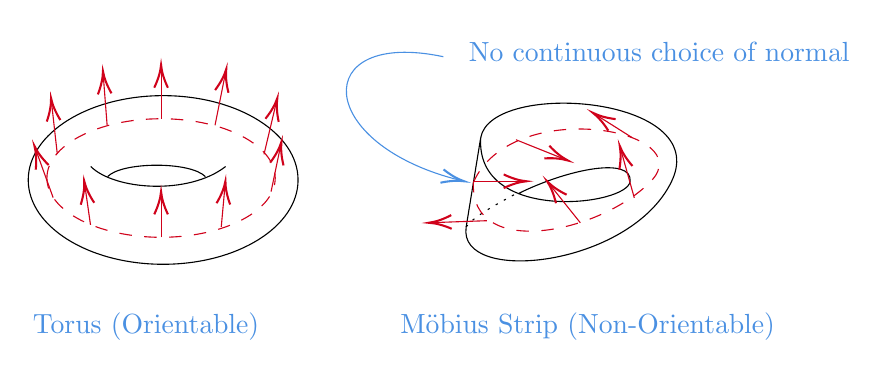
\begin{tikzpicture}[x=0.75pt,y=0.75pt,yscale=-1,xscale=1]
%uncomment if require: \path (0,202); %set diagram left start at 0, and has height of 202

%Curve Lines [id:da05527802912152291] 
\draw    (140.12,72.88) .. controls (151.5,84.25) and (187.25,86.85) .. (205.12,72.88) ;
%Curve Lines [id:da5225555438075742] 
\draw    (195.37,77.75) .. controls (187.9,70.28) and (155.07,70.6) .. (148.25,77.75) ;
%Shape: Ellipse [id:dp3063344683235558] 
\draw   (110,79.38) .. controls (110,56.94) and (139.1,38.75) .. (175,38.75) .. controls (210.9,38.75) and (240,56.94) .. (240,79.38) .. controls (240,101.81) and (210.9,120) .. (175,120) .. controls (139.1,120) and (110,101.81) .. (110,79.38) -- cycle ;
%Straight Lines [id:da6184709043628867] 
\draw [color={rgb, 255:red, 208; green, 2; blue, 27 }  ,draw opacity=1 ]   (223.6,67) -- (229.54,41.95) ;
\draw [shift={(230,40)}, rotate = 103.34] [color={rgb, 255:red, 208; green, 2; blue, 27 }  ,draw opacity=1 ][line width=0.75]    (10.93,-3.29) .. controls (6.95,-1.4) and (3.31,-0.3) .. (0,0) .. controls (3.31,0.3) and (6.95,1.4) .. (10.93,3.29)   ;
%Straight Lines [id:da24851539996932948] 
\draw    (328,59) -- (321,102) ;
%Curve Lines [id:da7319120828999304] 
\draw    (328,59) .. controls (333,31) and (439.8,38.6) .. (420,80) .. controls (400.2,121.4) and (316.6,130.2) .. (321,102) ;
%Curve Lines [id:da955357858158234] 
\draw    (328,59) .. controls (325.4,100.6) and (399,91.8) .. (400,80) .. controls (401,68.2) and (370.6,73.8) .. (346,86) ;
%Curve Lines [id:da1240095272344981] 
\draw  [dash pattern={on 0.84pt off 2.51pt}]  (321,102) .. controls (324.6,97) and (335,91.4) .. (345,86) ;
%Shape: Ellipse [id:dp5049740326726107] 
\draw  [color={rgb, 255:red, 208; green, 2; blue, 27 }  ,draw opacity=1 ][dash pattern={on 4.5pt off 4.5pt}] (119,78.44) .. controls (119,62.66) and (143.62,49.88) .. (174,49.88) .. controls (204.38,49.88) and (229,62.66) .. (229,78.44) .. controls (229,94.21) and (204.38,107) .. (174,107) .. controls (143.62,107) and (119,94.21) .. (119,78.44) -- cycle ;
%Straight Lines [id:da9359578969630631] 
\draw [color={rgb, 255:red, 208; green, 2; blue, 27 }  ,draw opacity=1 ]   (200,53) -- (205.01,27.96) ;
\draw [shift={(205.4,26)}, rotate = 101.31] [color={rgb, 255:red, 208; green, 2; blue, 27 }  ,draw opacity=1 ][line width=0.75]    (10.93,-3.29) .. controls (6.95,-1.4) and (3.31,-0.3) .. (0,0) .. controls (3.31,0.3) and (6.95,1.4) .. (10.93,3.29)   ;
%Straight Lines [id:da3289515902723321] 
\draw [color={rgb, 255:red, 208; green, 2; blue, 27 }  ,draw opacity=1 ]   (174,49.88) -- (174,26) ;
\draw [shift={(174,24)}, rotate = 90] [color={rgb, 255:red, 208; green, 2; blue, 27 }  ,draw opacity=1 ][line width=0.75]    (10.93,-3.29) .. controls (6.95,-1.4) and (3.31,-0.3) .. (0,0) .. controls (3.31,0.3) and (6.95,1.4) .. (10.93,3.29)   ;
%Straight Lines [id:da09641925370320403] 
\draw [color={rgb, 255:red, 208; green, 2; blue, 27 }  ,draw opacity=1 ]   (148,52.88) -- (146.15,28.99) ;
\draw [shift={(146,27)}, rotate = 85.58] [color={rgb, 255:red, 208; green, 2; blue, 27 }  ,draw opacity=1 ][line width=0.75]    (10.93,-3.29) .. controls (6.95,-1.4) and (3.31,-0.3) .. (0,0) .. controls (3.31,0.3) and (6.95,1.4) .. (10.93,3.29)   ;
%Straight Lines [id:da2908901884677755] 
\draw [color={rgb, 255:red, 208; green, 2; blue, 27 }  ,draw opacity=1 ]   (124,66.88) -- (121.22,41.99) ;
\draw [shift={(121,40)}, rotate = 83.63] [color={rgb, 255:red, 208; green, 2; blue, 27 }  ,draw opacity=1 ][line width=0.75]    (10.93,-3.29) .. controls (6.95,-1.4) and (3.31,-0.3) .. (0,0) .. controls (3.31,0.3) and (6.95,1.4) .. (10.93,3.29)   ;
%Straight Lines [id:da23254355767226764] 
\draw [color={rgb, 255:red, 208; green, 2; blue, 27 }  ,draw opacity=1 ]   (122,87.88) -- (113.68,64.88) ;
\draw [shift={(113,63)}, rotate = 70.11] [color={rgb, 255:red, 208; green, 2; blue, 27 }  ,draw opacity=1 ][line width=0.75]    (10.93,-3.29) .. controls (6.95,-1.4) and (3.31,-0.3) .. (0,0) .. controls (3.31,0.3) and (6.95,1.4) .. (10.93,3.29)   ;
%Straight Lines [id:da5510348186397793] 
\draw [color={rgb, 255:red, 208; green, 2; blue, 27 }  ,draw opacity=1 ]   (140,101) -- (137.28,81.98) ;
\draw [shift={(137,80)}, rotate = 81.87] [color={rgb, 255:red, 208; green, 2; blue, 27 }  ,draw opacity=1 ][line width=0.75]    (10.93,-3.29) .. controls (6.95,-1.4) and (3.31,-0.3) .. (0,0) .. controls (3.31,0.3) and (6.95,1.4) .. (10.93,3.29)   ;
%Straight Lines [id:da05975983118898509] 
\draw [color={rgb, 255:red, 208; green, 2; blue, 27 }  ,draw opacity=1 ]   (174,107) -- (174,87) ;
\draw [shift={(174,85)}, rotate = 90] [color={rgb, 255:red, 208; green, 2; blue, 27 }  ,draw opacity=1 ][line width=0.75]    (10.93,-3.29) .. controls (6.95,-1.4) and (3.31,-0.3) .. (0,0) .. controls (3.31,0.3) and (6.95,1.4) .. (10.93,3.29)   ;
%Straight Lines [id:da44294131424364247] 
\draw [color={rgb, 255:red, 208; green, 2; blue, 27 }  ,draw opacity=1 ]   (203,102) -- (204.82,81.99) ;
\draw [shift={(205,80)}, rotate = 95.19] [color={rgb, 255:red, 208; green, 2; blue, 27 }  ,draw opacity=1 ][line width=0.75]    (10.93,-3.29) .. controls (6.95,-1.4) and (3.31,-0.3) .. (0,0) .. controls (3.31,0.3) and (6.95,1.4) .. (10.93,3.29)   ;
%Straight Lines [id:da8437130662647478] 
\draw [color={rgb, 255:red, 208; green, 2; blue, 27 }  ,draw opacity=1 ]   (227,85) -- (231.59,62.96) ;
\draw [shift={(232,61)}, rotate = 101.77] [color={rgb, 255:red, 208; green, 2; blue, 27 }  ,draw opacity=1 ][line width=0.75]    (10.93,-3.29) .. controls (6.95,-1.4) and (3.31,-0.3) .. (0,0) .. controls (3.31,0.3) and (6.95,1.4) .. (10.93,3.29)   ;
%Curve Lines [id:da18056505853386673] 
\draw [color={rgb, 255:red, 208; green, 2; blue, 27 }  ,draw opacity=1 ] [dash pattern={on 4.5pt off 4.5pt}]  (324.5,80.5) .. controls (343,38.6) and (434.2,55) .. (410,80) .. controls (385.8,105) and (322.6,118.2) .. (324.5,80.5) -- cycle ;
%Straight Lines [id:da16920344082056782] 
\draw [color={rgb, 255:red, 208; green, 2; blue, 27 }  ,draw opacity=1 ]   (402,88) -- (395.54,64.93) ;
\draw [shift={(395,63)}, rotate = 74.36] [color={rgb, 255:red, 208; green, 2; blue, 27 }  ,draw opacity=1 ][line width=0.75]    (10.93,-3.29) .. controls (6.95,-1.4) and (3.31,-0.3) .. (0,0) .. controls (3.31,0.3) and (6.95,1.4) .. (10.93,3.29)   ;
%Straight Lines [id:da5162379834614435] 
\draw [color={rgb, 255:red, 208; green, 2; blue, 27 }  ,draw opacity=1 ]   (376,100) -- (361.25,81.56) ;
\draw [shift={(360,80)}, rotate = 51.34] [color={rgb, 255:red, 208; green, 2; blue, 27 }  ,draw opacity=1 ][line width=0.75]    (10.93,-3.29) .. controls (6.95,-1.4) and (3.31,-0.3) .. (0,0) .. controls (3.31,0.3) and (6.95,1.4) .. (10.93,3.29)   ;
%Straight Lines [id:da15822931325348022] 
\draw [color={rgb, 255:red, 208; green, 2; blue, 27 }  ,draw opacity=1 ]   (331,99) -- (305,99.93) ;
\draw [shift={(303,100)}, rotate = 357.95] [color={rgb, 255:red, 208; green, 2; blue, 27 }  ,draw opacity=1 ][line width=0.75]    (10.93,-3.29) .. controls (6.95,-1.4) and (3.31,-0.3) .. (0,0) .. controls (3.31,0.3) and (6.95,1.4) .. (10.93,3.29)   ;
%Straight Lines [id:da3341110759567949] 
\draw [color={rgb, 255:red, 208; green, 2; blue, 27 }  ,draw opacity=1 ]   (325,80) -- (348,80) ;
\draw [shift={(350,80)}, rotate = 180] [color={rgb, 255:red, 208; green, 2; blue, 27 }  ,draw opacity=1 ][line width=0.75]    (10.93,-3.29) .. controls (6.95,-1.4) and (3.31,-0.3) .. (0,0) .. controls (3.31,0.3) and (6.95,1.4) .. (10.93,3.29)   ;
%Straight Lines [id:da17563158134376344] 
\draw [color={rgb, 255:red, 208; green, 2; blue, 27 }  ,draw opacity=1 ]   (345,60) -- (368.14,69.26) ;
\draw [shift={(370,70)}, rotate = 201.8] [color={rgb, 255:red, 208; green, 2; blue, 27 }  ,draw opacity=1 ][line width=0.75]    (10.93,-3.29) .. controls (6.95,-1.4) and (3.31,-0.3) .. (0,0) .. controls (3.31,0.3) and (6.95,1.4) .. (10.93,3.29)   ;
%Straight Lines [id:da5963965638960156] 
\draw [color={rgb, 255:red, 208; green, 2; blue, 27 }  ,draw opacity=1 ]   (401,59) -- (383.69,48.07) ;
\draw [shift={(382,47)}, rotate = 32.28] [color={rgb, 255:red, 208; green, 2; blue, 27 }  ,draw opacity=1 ][line width=0.75]    (10.93,-3.29) .. controls (6.95,-1.4) and (3.31,-0.3) .. (0,0) .. controls (3.31,0.3) and (6.95,1.4) .. (10.93,3.29)   ;
%Curve Lines [id:da24333526890590362] 
\draw [color={rgb, 255:red, 74; green, 144; blue, 226 }  ,draw opacity=1 ]   (310,20) .. controls (245.32,6.27) and (247.31,62.43) .. (318.92,79.74) ;
\draw [shift={(320,80)}, rotate = 193.17] [color={rgb, 255:red, 74; green, 144; blue, 226 }  ,draw opacity=1 ][line width=0.75]    (10.93,-3.29) .. controls (6.95,-1.4) and (3.31,-0.3) .. (0,0) .. controls (3.31,0.3) and (6.95,1.4) .. (10.93,3.29)   ;

% Text Node
\draw (111,142) node [anchor=north west][inner sep=0.75pt]  [color={rgb, 255:red, 74; green, 144; blue, 226 }  ,opacity=1 ] [align=left] {Torus (Orientable)};
% Text Node
\draw (288,142) node [anchor=north west][inner sep=0.75pt]  [color={rgb, 255:red, 74; green, 144; blue, 226 }  ,opacity=1 ] [align=left] {Möbius Strip (Non-Orientable)};
% Text Node
\draw (321,12) node [anchor=north west][inner sep=0.75pt]  [color={rgb, 255:red, 74; green, 144; blue, 226 }  ,opacity=1 ] [align=left] {No continuous choice of normal};


\end{tikzpicture}


\end{center}

\section{Geometry of Surfaces in \texorpdfstring{$\R^3$}{R3}}

\subsection{First Fundamental Form}

Having developed some ways to discuss surfaces particularly in $\R^3$, we are going to start discussing more geometric notions such as length and angles.

Recall that for a curve $\gamma: (a, b) \rightarrow \R^3$, the length of $\gamma$ is given by
$$
L(\gamma) = \int_a^b \norm{\gamma'(t)} \dd t.
$$
Since this is independent of paramterisation\footnote{Feel free to check this}, we can naturally parameterise a curve with respect to arc length (as long as $\gamma'(t) \neq 0$). Now, given a curve on some smooth surface in $\R^3$, we want to find a nice way to compute lengths.

let $\Sigma$ be a smoth surface in $\R^3$, and let $\sigma: V \rightarrow U \subseteq \Sigma$ be an allowable parameterisation. Let $\gamma: (a, b) \rightarrow \R^3$ be smooth and have its image be contained in $U$. Then writing $\gamma(t) = \sigma(u(t), v(t))$, and so $\gamma'(t) = \sigma_u u'(t) + \sigma_v v'(t)$, giving
$$
\norm{\gamma'(t)} = E u'(t)^2 + 2F u'(t) v(t) + Gv'(t)^2,
$$
for functions
$$
E = \langle \sigma_u, \sigma_u\rangle; \quad F = \langle \sigma_u, \sigma_v \rangle = \langle \sigma_v, \sigma_u \rangle; \quad G = \langle \sigma_v, \sigma_v \rangle,
$$
where $\langle \cdot, \cdot \rangle$ is our Euclidean inner product. These values encapsulate the notion of length for our surface.

\begin{definition}[First Fundamental Form]
    The \vocab{first fundamental form} of $\Sigma$ in the parameterisation $\sigma$ is the expression
    $$
    E \dd u^2 + 2F \dd u \dd v + G \dd v^2.
    $$
\end{definition}

Note that if $\gamma$ has image in the image of $\sigma$, then
$$
L(\gamma) = \int_a^b \sqrt{E (u')^2 + 2F u' v' + G(v')^2} \dd t.
$$
With length encapsulated by the first fundamental form, we get a nice way to capture when two surfaces (locally) have the same `geometry' in a \emph{length} sense.

\begin{definition}[Isometric]
    Let $\Sigma, \Sigma'$ be smooth surfaces in $\R^3$. We say that they are \vocab{isometric} if there exists a diffeomorphism $f: \Sigma \rightarrow \Sigma'$ that preserves the length of al curves.
\end{definition}
\begin{definition}[Locally Isometric]
    We say that $\Sigma, \Sigma'$ are \emph{locally isometric} near points $p \in \Sigma$ and $q \in \Sigma'$ if there exists open neighbourhoods $U$ of $p$ and $V$ of $q$ such that $U$ and $V$ are isometric.
\end{definition}
\begin{lemma}
    Smooth surfaces $\Sigma, \Sigma'$ in $\R^3$ are locally isometric near $p \in \Sigma$ and $q \in \Sigma'$ if and only if there exist allowable parameterisations $\sigma: V \rightarrow U \subseteq \Sigma$ and $\sigma': V \rightarrow U' \subseteq \Sigma'$ such that the first fundamental forms are equivalent. 
\end{lemma}
\begin{proof}
    Omitted.
\end{proof}

\subsection{Area}

With length pinned down by the first fundamental form, it's not too hard to pin down area. 

Recall that a parallelogram spanned by two vectors $v, w$ has area $|v \times w| = \langle v, v \rangle \langle w, w \rangle - \langle v, w \rangle^2$. So if we have an allowable parameterisation $\sigma: V \rightarrow U \subseteq \Sigma$ with $\sigma(0) = p$, and consider $\sigma_u, \sigma_v \in T_p \Sigma$, the square of the area of the infinitesimal parallelogram spanned by $\sigma_u, \sigma_v$ is given by
$$
\langle \sigma_u, \sigma_u \rangle \langle \sigma_v, \sigma_v \rangle - \langle \sigma_u, \sigma_v \rangle^2 = EG - F^2.
$$
This gives us a sensible way to define area.

\begin{definition}[Area]
    Let $\Sigma$ be a smooth surface in $\R^3$, and let $\sigma: V \rightarrow U \subseteq \Sigma$ be an allowable parameterisation. Then
    $$
\operatorname{area}(U) = \int_V \sqrt{EG - F^2} \dd u \dd v.
    $$
\end{definition}

\subsection{Second Fundamental Form}


Intuitively, the first fundamental form pins down how length works along our surface. We now, through the second fundamental form, will try to pin down how \emph{curved} our surface is (as an embedding of $\R^3$).

We are (informally) going to look at curvature at a point as measuring how much we deviate from the tangent plane by moving a small amount away from our point.

\begin{center}
    

\tikzset{every picture/.style={line width=0.75pt}} %set default line width to 0.75pt        

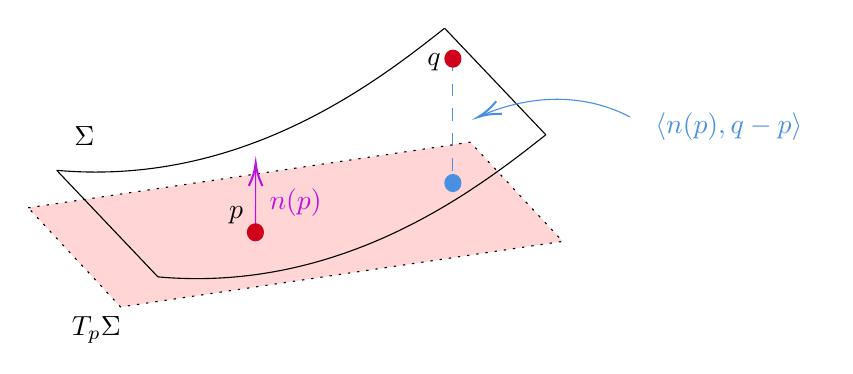
\begin{tikzpicture}[x=0.75pt,y=0.75pt,yscale=-1,xscale=1]
%uncomment if require: \path (0,459); %set diagram left start at 0, and has height of 459

%Shape: Parallelogram [id:dp7900821750552607] 
\draw  [fill={rgb, 255:red, 255; green, 179; blue, 179 }  ,fill opacity=0.55 ][dash pattern={on 0.84pt off 2.51pt}] (6,89.18) -- (218.98,57.58) -- (263.5,105.36) -- (50.51,136.96) -- cycle ;
%Straight Lines [id:da32794339542910955] 
\draw [color={rgb, 255:red, 74; green, 144; blue, 226 }  ,draw opacity=1 ] [dash pattern={on 4.5pt off 4.5pt}]  (210.61,17.34) -- (210.61,77.25) ;
%Straight Lines [id:da9843969307420661] 
\draw    (19.72,71.13) -- (68.48,122.47) ;
%Curve Lines [id:da6590186468140269] 
\draw    (68.48,122.47) .. controls (157.86,130.43) and (222.87,79.69) .. (255.37,54.01) ;
%Curve Lines [id:da12117500145497906] 
\draw    (19.72,71.13) .. controls (109.11,79.09) and (174.11,28.34) .. (206.62,2.67) ;
%Straight Lines [id:da969061893759412] 
\draw    (206.62,2.67) -- (255.37,54.01) ;
%Shape: Ellipse [id:dp3759846798866977] 
\draw  [draw opacity=0][fill={rgb, 255:red, 208; green, 2; blue, 27 }  ,fill opacity=1 ] (206.47,17.34) .. controls (206.47,14.93) and (208.33,12.98) .. (210.61,12.98) .. controls (212.89,12.98) and (214.74,14.93) .. (214.74,17.34) .. controls (214.74,19.75) and (212.89,21.71) .. (210.61,21.71) .. controls (208.33,21.71) and (206.47,19.75) .. (206.47,17.34) -- cycle ;
%Shape: Ellipse [id:dp4473354880432048] 
\draw  [draw opacity=0][fill={rgb, 255:red, 74; green, 144; blue, 226 }  ,fill opacity=1 ] (206.47,77.25) .. controls (206.47,74.84) and (208.33,72.88) .. (210.61,72.88) .. controls (212.89,72.88) and (214.74,74.84) .. (214.74,77.25) .. controls (214.74,79.66) and (212.89,81.61) .. (210.61,81.61) .. controls (208.33,81.61) and (206.47,79.66) .. (206.47,77.25) -- cycle ;
%Straight Lines [id:da32292000427802847] 
\draw [color={rgb, 255:red, 189; green, 16; blue, 224 }  ,draw opacity=1 ]   (115.47,100.99) -- (115.6,69.71) ;
\draw [shift={(115.61,67.71)}, rotate = 90.24] [color={rgb, 255:red, 189; green, 16; blue, 224 }  ,draw opacity=1 ][line width=0.75]    (10.93,-3.29) .. controls (6.95,-1.4) and (3.31,-0.3) .. (0,0) .. controls (3.31,0.3) and (6.95,1.4) .. (10.93,3.29)   ;
%Shape: Ellipse [id:dp3469616434750329] 
\draw  [draw opacity=0][fill={rgb, 255:red, 208; green, 2; blue, 27 }  ,fill opacity=1 ] (111.33,100.99) .. controls (111.33,98.58) and (113.18,96.63) .. (115.47,96.63) .. controls (117.75,96.63) and (119.6,98.58) .. (119.6,100.99) .. controls (119.6,103.4) and (117.75,105.36) .. (115.47,105.36) .. controls (113.18,105.36) and (111.33,103.4) .. (111.33,100.99) -- cycle ;
%Curve Lines [id:da36924394958097206] 
\draw [color={rgb, 255:red, 74; green, 144; blue, 226 }  ,draw opacity=1 ]   (296,45.42) .. controls (271.44,32.74) and (245.33,35.68) .. (224.46,44.71) ;
\draw [shift={(222.87,45.42)}, rotate = 335.61] [color={rgb, 255:red, 74; green, 144; blue, 226 }  ,draw opacity=1 ][line width=0.75]    (10.93,-3.29) .. controls (6.95,-1.4) and (3.31,-0.3) .. (0,0) .. controls (3.31,0.3) and (6.95,1.4) .. (10.93,3.29)   ;

% Text Node
\draw (101.48,87.28) node [anchor=north west][inner sep=0.75pt]  [color={rgb, 255:red, 0; green, 0; blue, 0 }  ,opacity=1 ]  {$p$};
% Text Node
\draw (27,48.81) node [anchor=north west][inner sep=0.75pt]  [color={rgb, 255:red, 0; green, 0; blue, 0 }  ,opacity=1 ]  {$\Sigma $};
% Text Node
\draw (25.76,140.4) node [anchor=north west][inner sep=0.75pt]  [color={rgb, 255:red, 0; green, 0; blue, 0 }  ,opacity=1 ]  {$T_{p} \Sigma $};
% Text Node
\draw (197,13.81) node [anchor=north west][inner sep=0.75pt]  [color={rgb, 255:red, 0; green, 0; blue, 0 }  ,opacity=1 ]  {$q$};
% Text Node
\draw (121,78.81) node [anchor=north west][inner sep=0.75pt]  [color={rgb, 255:red, 189; green, 16; blue, 224 }  ,opacity=1 ]  {$n( p)$};
% Text Node
\draw (297,42) node [anchor=north west][inner sep=0.75pt]  [color={rgb, 255:red, 74; green, 144; blue, 226 }  ,opacity=1 ] [align=left] {\begin{minipage}[lt]{67.96pt}\setlength\topsep{0pt}
\begin{center}
$\displaystyle \langle n( p) ,q-p\rangle $
\end{center}

\end{minipage}};


\end{tikzpicture}

\end{center}

Let $\Sigma$ be a smooth surface in $\R^3$, and let $\sigma: V \rightarrow U \subseteq \Sigma$ be an allowable parameterisation. Consider a point $p = \sigma(u, v)$, and some nearby point $q = \sigma(u + h, v + \ell)$. Then by Taylor's theorem we have
\begin{align*}
\sigma(u + h, v + \ell) &= \sigma(u, v) + h \sigma_u(u, v) + \ell \sigma_v(u, v) \\
&\ + \frac{1}{2}\left(h^2 \sigma_uu(u, v) + 2 h\ell \sigma_{uv}(u, v) + \ell^2 \sigma_{vv}(u, v)\right)\\&\ + O(h^3, \ell^3).
\end{align*}
Recalling that the tangent plane is given by $T_p\Sigma = \operatorname{span}\{\sigma_u, \sigma_v\}$, we get the perpendicular distance from $q = \sigma(u + h, v+\ell)$ to the affine tangent plane $T_p\Sigma + p$ is given by
\begin{align*}
    \langle n, \sigma(u + h, v + \ell) - \sigma(u, v)\rangle &= \frac{1}{2}\left(\langle n, \sigma_{uu} \rangle h^2 + 2 \langle h, \sigma_{uv}\rangle h \ell + \langle n, \sigma_{vv} \rangle \ell^2\right)\\&\  + O(h^3, l^3). 
\end{align*}
and so we can see that these inner products give us this difference. This inspires our definition of the second fundamental form.

\begin{definition}[Second Fundamental Form]
    The \vocab{second fundamental form} of $\Sigma$ in the allowable parameterisation $\sigma$ is
    $$
    L \dd u^2 + 2M \dd u \dd v + N \dd v^2
    $$
    where $L = \langle n, \sigma_{uu} \rangle$, $M =  \langle n, \sigma_{uv} \rangle$, and $N = \langle n, \sigma_{vv} \rangle$, and $n$ is the unit normal given by $n = \frac{\sigma_u \times \sigma_v}{\norm{\sigma_u \times \sigma_v}}$.
\end{definition}

We will say more about how this relates to curvature in the coming sections. It's good to know (but not proven in this course) that the two fundamental forms completely determine a smooth oriented connected surface in $\R^3$, up to rigid motion. This is the \emph{fundamental theorem of surfaces in $\R^3$}.

\subsection{The Gauss Map and Curvature}

We are now going to define what our notion of curvature actually is. This is done using the \emph{Gauss map}.

\begin{definition}[Gauss Map]
    Let $\Sigma$ be a smooth oriented surface in $\R^3$. The \vocab{Gauss map} $n : \Sigma \rightarrow S^2$ is the map $p \mapsto n(p)$, where the normal vector is normalised and hence lies in the unit sphere.
\end{definition}

% \begin{lemma}
%     The Gauss map is smooth.
% \end{lemma}

% \begin{proof}
%     Let $p \in \Sigma$ and let $\sigma: V \rightarrow U \subseteq \Sigma$ with $p \in U$ be allowable and compatible with our chosen orientation. Then
%     $$
%     n(p) = \frac{\sigma_u \times \sigma_v}{\norm{\sigma_u \times \sigma_v}}.
%     $$
%     Since $\sigma$ is allowable, the denominator is non-vanishing and hence $n(p)$ is smooth as required.
% \end{proof}

\begin{definition}[Gauss Curvature]
    Let $\Sigma$ be a smooth surface in $\R^3$. The \vocab{Gauss curvature $\kappa$} is $\kappa: \Sigma \rightarrow \R$ given by
    $$
    \kappa(p) = \det \left(\left.Dn\right|_p\right)
    $$
\end{definition}

We note that this is smooth since the Gauss map is smooth\footnote{Follows by writing down an expression for $n(p)$ and noting that it's the composition of smooth functions.} and is also always well defined even for non-orientable $\Sigma$, as $\Sigma$ is always locally orientable.

We can compute $\kappa$ by using the first and second fundamental forms, but it will require looking at these from a different perspective.

\subsubsection*{A Different Perspective on the Fundamental Forms}

The first fundamental form specifies 

We can compute what $\kappa$ is exactly.
{\color{red} TODO: FILL IN THE DETAILS}. And we arrive at
$$
\kappa = \frac{LN - M^2}{EG - F^2}.
$$


\begin{definition}
    A smooth surface in $\R^3$ with vanishing gauss curvature everywhere is called flat.
\end{definition}

\begin{definition}
    Let $\Sigma$ be a smooth surface in $\R^3$, and let $p \in \Sigma$. We say that
    \begin{enumerate}[label=(\roman*)]
        \item \vocab{elliptic} if $\kappa(p) > 0$;
        \item \vocab{hyperbolic} if $\kappa(p) < 0$;
        \item \vocab{parabolic} if $\kappa(p) = 0$.
    \end{enumerate}
\end{definition}

\begin{lemma}
    In sufficiently small nbhd of elliptic point, surface lies entirely to one side.
\end{lemma}
\begin{theorem}
    Compact smooth surface has elliptic point.
\end{theorem}

Now an interpretation of Gauss curvature. 

\begin{theorem}
    Let $\Sigma$ be a smooth surface in $\R^3$, and let $p \in \Sigma$ such that $\kappa(p) \neq 0$. Let $U$ be an open neighborhood of $p$, and a decreasing sequence $A_i \subseteq U$ of neighborhoods that `shrink to $p$' in the sense that for all $\varepsilon > 0$, $A_i \subseteq B(p, \varepsilon)$ for sufficiently large $i$. Then,
    $$
    |\kappa(p) | = \lim_{i \to \infty} \frac{\operatorname{area}_{S^2}(n(A_i))}{\operatorname{area}_\Sigma (A_i)}.
    $$
\end{theorem}
Informally, Gauss curvature is an infinitesimal measure of how much the Gauss map $n$ distorts area.

\begin{theorem}[Theorema Egregium]
    The gauss curvature is isometry invariant.
\end{theorem}

\begin{theorem}[Gauss-Bonnet]
    If $\Sigma$ is a compact smooth surface in $\R^3$, then
    $$
    \int_{\Sigma} \kappa \dd A_\Sigma = 2 \pi \chi(\Sigma).
    $$
\end{theorem}
% Let $\sigma: V \rightarrow U \subseteq \Sigma$ be an allowable parametrization, and let $p \in U$. Then noting that $\langle n, n\rangle = 0$, differentiating gives $\langle n, n_u \rangle = \langle n, n_v \rangle = 0$. Then since $\{\sigma_u, \sigma_v, n\}$ forms a basis, there's some $a, b, c, d$ such that
% $$
% n_u = a \sigma_u + b \sigma_v, \quad \text{and} \quad n_v = c \sigma_u + d \sigma_v.
% $$
% Now we also know that $\langle n, \sigma_u \rangle = 0$, and differentiating this gives $\langle n_u, \sigma_u\rangle + \langle n, \sigma_{uu} \rangle = 0$, that is, $\langle n_u, \sigma_u\rangle = -L$. Continuing on like this, we get
% $$
% -L = \langle n_u, \sigma_u \rangle, \quad -N = \langle n_v, \sigma_v \rangle, \quad -M = \langle n_v, \sigma_u \rangle.
% $$

% Other POV: FFF is bilinear form $I: T_p\Sigma \rightarrow T_p \Sigma$, so $I(v, w) = \langle v, w \rangle$. SFF is as before, and $I = (D\sigma)^T D\sigma$. $II = -(Dn)^T D\sigma$

% \section{Some Topological Surfaces}

% \subsection{}

% \appendix

% \section{The Inverse and Implicit Function Theorems}

% Test

\section{Geodesics}

\subsection{Definitions}

We are now going to discuss a particular geometric phenomena, \emph{geodesics}, which are curves with (in some sense) are the shortest path between points.

\begin{definition}[Energy]
    The \vocab{energy} of a curve $\gamma$ is given by 
    $$E(\gamma) = \int_a^b \norm{\gamma'(t)}^2 \dd t.$$
\end{definition}

\begin{definition}[One-Parameter Variation]
    Let $\gamma: [a, b] \rightarrow \Sigma$, where $\Sigma$ is a smooth surface in $\R^3$. A \vocab{one-parameter variation} (with fixed-endpoints) of $\gamma$ is a smooth map $\Gamma: (-\varepsilon, \varepsilon) \times [a, b] \rightarrow \Sigma$, such that if $\gamma_s = \gamma(s, \cdot)$, then $\gamma_0(t) = \gamma(t)$ and $\gamma_s(a)$ and $\gamma_s(b)$ are independent of $s$.
\end{definition}

\begin{definition}[Geodesic]
    A smooth curve $\gamma: [a, b] \rightarrow \Sigma$ is a \vocab{geodesic} if\footnote{Alternatively, $\gamma$ is a critical point of the energy functional on curves from $\gamma(a)$ to $\gamma(b)$.}, for every variation $(\gamma_s)$ of $\gamma$ with fixed endpoints, we have $\left.\frac{\dd}{\dd s}\right|_{s = 0} E(\gamma_s) = 0$.
\end{definition}

\subsection{The Geodesic Equations}

So how do we actually find geodesics? It turns out to be \emph{relatively} easy, using the geodesic equations.

Suppose we have some curve $\gamma$ with image contained in an allowable parameterisation $\sigma$. Then for sufficiently small $s$, we can write $\gamma_s(t) = \sigma(u(s, t), v(s, t))$. 
Now let the first fundamental form with respect to $\sigma$ be
$$
E \dd u ^2 + 2F \dd u \dd v + G \dd v^2.
$$
Then by definition,
$$
E(\gamma_s) = \int_a^b E \dot{u}^2 + 2F \dot{u} \dot{v} + G \dot{v}^2 \dd t.
$$
Differentiating under the integral sign and integrating by parts, we get
$$
\left.\frac{\dd}{\dd s} E(\gamma_s) \right|_{s = 0} = \left.\int_a^b A \frac{\partial u}{\partial s} + B \frac{\partial v}{\partial s} \dd t \right|_{s = 0}
$$
where
\begin{align*}
    A &= E_u \dot{u}^2 + 2F_u \dot{u} \dot{v} + G_u \dot{v}^2 - 2 \frac{\dd}{\dd t} (E \dot{u} + F \dot{v}) \\
    B &= E_v \dot{u}^2 + 2F_v \dot{u} \dot{v} + G_v \dot{v}^2 - 2 \frac{\dd}{\dd t}(F \dot{u} + G\dot{v})
\end{align*}
These give us the \emph{geodesic equations}.

\begin{theorem}[Geodesic Equations]
    A smooth curve $\gamma(t) = \sigma(u(t), v(t))$ is a geodesic if and only if it satisfies the geodesic equations
    \begin{align*}
        \frac{\dd}{\dd t} (E \dot{u} + F \dot{v}) &= \frac{
        E_u \dot{u}^2 + 2F_u \dot{u} \dot{v} + G_u \dot{v}^2}{2} \\
        \frac{\dd}{\dd t}(F \dot{u} + G\dot{v})  &= \frac{E_v \dot{u}^2 + 2F_v \dot{u} \dot{v} + G_v \dot{v}^2}{2}
    \end{align*}
\end{theorem}

Unlike length, energy is sensitive to reparameterisation, but Cauchy-Schwarz gives us that $L(\gamma)^2 \leq E(\gamma) (b - a)$, with equality if and only if $\gamma$ is parameterized proportional to arc length.

\begin{corollary}
    If $\gamma$ has constant speed and locally minimizes length, then it is a geodesic. Further, if $\gamma$ minimizes energy globally, then it minimizes length globally and is parameterized with constant speed.
\end{corollary}

For some examples, the geodesics in the plane consist of straight lines, and the geodesics in the sphere consist of the curves of intersection between the sphere and planes through the origin.

In $\R^2$, the geodesics are not just locally shortest but they are also locally straightest. We would intuitively expect this to hold on other surfaces too. That is, we would expect the change in the tangent vector to be as small as possible subject to the constraint that we lie on the surface.

\begin{theorem}
    Let $\Sigma$ be a smooth surface in $\R^3$. A smooth curve $\gamma:[a, b] \rightarrow \Sigma$ is a geodesic if and only if $\ddot{\gamma}(t)$ is everywhere normal to the surface $\Sigma$.
\end{theorem}
\begin{proof}
    Omitted.
\end{proof}

\subsection{Surfaces of Revolution}

One common surface we come across is a surface of revolution, where we rotate say $\eta(u) = (f(u), 0, g(u))$ where $\nu$ is smooth and injective and $f(u)> 0$ about the $z$ axis.

\begin{definition}
A circle obtained by rotating a point of $\eta$ is called a \vocab{parallel}. A curve obtained by rotating $\eta$ itself by a fixed angle about the $z$-axis is a \vocab{meridian}.
\end{definition}

A plane in $\R^3$ containing the $z$-axis is a plane of symmetry, hence meridians are geodesics\footnote{\color{red} DETAIL HERE!}. Not all parallels are geodesics however.

\begin{lemma}
    A parallel given by $u = u_-0$ is a geodesic when parameterised at constant speed if and only if $f'(u_0) = 0$.
\end{lemma}
\begin{proof}
    Omitted.
\end{proof}

Consider a curve $\gamma(t)$ on $\Sigma$, making an angle $\theta$ with a parallel of radius $\rho = f$.

\begin{theorem}[Clairaut's Relation]
    If $\gamma$ is a geodesic, then $\rho \cos \theta$ is constant along $\gamma$.
\end{theorem}

\subsection{Surfaces of Constant Curvature}

Our result looks like this:

\begin{proposition}
    Let $\Sigma$ be a smooth surface in $\R^3$. Then,
    \begin{enumerate}[label=(\roman*)]
        \item If $\kappa \equiv 0$, then $\Sigma$ is locally isometric to $(\R^2, \dd u^2 + \dd v^2)$
        \item If $\kappa \equiv 1$, then $\Sigma$ is locally isometric to $(S^2, \dd u^2 + \cos^2 u  \dd v^2)$.
    \end{enumerate}
\end{proposition}

\subsection{Riemannian Metrics}

\subsection{The Length Metric}

So far, the geometry of our surfaces has been induced by the space that surface has been embed in (which has so far been $\R^3$). Of course, it's possible to do geometry on surfaces that do not arise in this way. 
One way of specifying the geometry of a surface is with a \emph{Riemannian metric}.

\begin{definition}[Riemannian Metric]
    Let $V \subseteq \R^2$ be an open set. An (abstract) \vocab{Riemannian metric} is a smooth map from $V$ to the set of positive definite symmetric billinear forms, given by
    $$
    v \mapsto \begin{pmatrix}
        E(v) & F(v) \\
        F(v) & G(v)
    \end{pmatrix},
    $$
    such that $E, G, EG - F^2 > 0$.
\end{definition}

If $v$ is a vector at $p \in C$, we can compute its infinitesmal length by
$$
\norm{v}^2 = v^\top \begin{pmatrix}
    E(v) & F(v) \\ F(v) & G(v)
\end{pmatrix} v.
$$
So, if $\gamma: [a, b] \rightarrow V$ is smooth,
$$
L(\gamma) = \int_a^b \sqrt{E \dot{u}^2 + 2F \dot{u}\dot{v} + G \dot{v}^2} \dd t,
$$
where $\gamma(t) = (u(t), v(t))$.

% \end{multicols*}
\end{document}
